\documentclass[12pt]{article}
\usepackage[utf8]{inputenc}
\usepackage[margin=1in]{geometry}
\usepackage{amsmath,amssymb,amsthm}
\usepackage{natbib}
% Ensure that a leftover \NAT@force@numbers from previous bib runs cannot force numeric citations
\makeatletter
\providecommand\NAT@force@numbers{}
\makeatother
\usepackage[hypertexnames=false]{hyperref}
\usepackage{graphicx}
\usepackage{booktabs}
\usepackage{float}
\usepackage{setspace}
\usepackage{enumitem}

\doublespacing

\title{Replication and Extension of the Quantitative Microfounded Model\\for the Integrated Policy Framework in Julia\\\vspace{0.5cm}\large{Technical Appendix} \\\vspace{0.5cm} \it Preliminary - Please do not cite}

\author{M\'aty\'as Farkas\thanks{mfarkas@imf.org}\\
{\small {International Monetary Fund}}}
\date{\today}
\date{\vspace{0.0cm}   First version: January 13, 2025} 

% Prevent stale aux/bibtex artifacts from forcing numeric citations
\makeatletter
\providecommand\NAT@force@numbers{}
\let\NAT@force@numbers\relax
\makeatother

\begin{document}

\maketitle

\begin{abstract}
\noindent This technical appendix documents the replication and extension of the Quantitative Microfounded Model for the Integrated Policy Framework (QMIPF) originally developed by \citet{adrian2021quantitative} in Julia using the MacroModelling.jl package. We provide a comprehensive derivation of the non-linear model equations, detail implementation differences from the original Dynare specification, and demonstrate successful convergence of the Stochastic Extended Path (SEP) solver for computing non-linear impulse response functions. The Julia implementation achieves comparable accuracy to first-order perturbation methods while enabling non-linear solution techniques essential for analyzing financial stability and capital flow management policies.
\end{abstract}

\vspace{1cm}

\tableofcontents

\newpage

\section{Introduction}

The Integrated Policy Framework (IPF), developed by the International Monetary Fund, provides a coherent analytical framework for understanding how emerging market and developing economy policymakers can deploy multiple policy tools---monetary policy, foreign exchange intervention (FXI), and capital flow management measures (CFMs)---to achieve macroeconomic stability \citep{adrian2020conceptual}. The Quantitative Microfounded Model for the Integrated Policy Framework (QMIPF) by \citet{adrian2021quantitative} represents a significant advancement in operationalizing this framework by providing a fully microfounded dynamic stochastic general equilibrium (DSGE) model suitable for quantitative policy analysis.

This technical appendix documents our replication of the QMIPF model in Julia using the MacroModelling.jl package \citep{MacroModellingJL}. Our implementation achieves three key objectives: (1) faithful replication of the core theoretical structure, (2) successful steady-state computation and first-order perturbation solution, and (3) operational non-linear solution methods via the Stochastic Extended Path algorithm.

The remainder of this appendix is organized as follows. Section \ref{sec:literature} provides a brief literature review situating the QMIPF model within the broader DSGE and open economy macroeconomics literature. Section \ref{sec:model} presents the complete theoretical derivation of the model equations. Section \ref{sec:implementation} details the Julia implementation and documents key differences from the original Dynare specification. Section \ref{sec:numerical} discusses the numerical solution methods, with particular emphasis on the SEP algorithm. Section \ref{sec:results} presents calibration and validation results. Section \ref{sec:conclusion} concludes.

\section{Literature Review}\label{sec:literature}

\subsection{The Integrated Policy Framework}

The QMIPF model builds upon the IMF's Integrated Policy Framework research agenda, which seeks to provide coherent guidance on the coordinated use of multiple policy instruments in open economies. The conceptual foundations were laid out in \citet{adrian2020conceptual}, which articulated the theoretical rationale for deploying FXI and CFMs alongside conventional monetary policy under specific circumstances: shallow financial markets, exchange rate pass-through to inflation, currency mismatches on balance sheets, and imperfectly anchored inflation expectations.

The first quantitative implementation, the QIPF model \citep{adrian2020quantitative}, developed an empirically-oriented New Keynesian framework demonstrating that FXI and CFMs can improve policy tradeoffs and reduce sudden stop risks. The QMIPF model \citep{adrian2021quantitative} extends this work by providing full microfoundations, introducing nonlinear balance sheet channels, and allowing for more detailed analysis of financial stability concerns.

\subsection{Open Economy DSGE Models}

The QMIPF model draws on the rich tradition of open economy New Keynesian models pioneered by \citet{gali2005monetary}, who extended the canonical closed economy framework to incorporate international linkages through import content in consumption, terms of trade dynamics, and uncovered interest parity conditions. The model structure adopted by \citet{adrian2021quantitative} follows this tradition while incorporating additional financial frictions and policy instruments relevant for emerging market economies.

A key innovation in the QMIPF model is its treatment of the uncovered interest parity (UIP) condition. While standard formulations impose perfect capital mobility, the QMIPF specification incorporates endogenous risk premia depending on net foreign asset positions, following the insights of \citet{schmitt2003closing} on the role of debt-elastic interest rates in achieving model stationarity in open economy settings.

\subsection{Nominal Rigidities and Price Setting}

The model incorporates staggered price and wage setting following the framework developed by \citet{calvo1983staggered}. Under Calvo pricing, firms and unions face a constant probability $\xi_p$ and $\xi_w$ of being unable to re-optimize their prices and wages in a given period. This simple but tractable specification generates realistic inflation dynamics and allows for a clear characterization of monetary policy transmission mechanisms. The QMIPF model extends the standard Calvo framework by incorporating separate rigidities for domestic goods prices, import prices, and wages.

\subsection{Numerical Solution Methods}

Computing the QMIPF model's dynamics requires sophisticated numerical methods capable of handling its non-linearities and occasionally binding constraints. While first- and higher-order perturbation methods \citep{schmitt2004solving,andreasen2018pruning} provide accurate local approximations around the deterministic steady state, they can fail when stochastic steady states do not exist or when analyzing regimes far from the steady state.

The Stochastic Extended Path (SEP) algorithm provides an alternative global solution method particularly well-suited for models with strong non-linearities or occasionally binding constraints. Originally developed by \citet{fair1983solution} and extended by \citet{adjemian2013stochastic}, the SEP method computes perfect foresight paths under sequences of shocks while accounting for future uncertainty through Gaussian quadrature over possible shock realizations. \citet{adjemian2025stochastic} provide the most recent algorithmic refinements implemented in Dynare. Our Julia implementation adapts these techniques to the MacroModelling.jl framework.

\subsection{Contribution}

This replication contributes to the literature in three ways. First, we provide a complete, self-contained derivation of the QMIPF model equations suitable for researchers seeking to understand or extend the framework. Second, we document the practical implementation challenges and solutions for achieving numerical convergence. Third, we demonstrate that the Julia/MacroModelling.jl ecosystem provides a viable alternative to Dynare for implementing sophisticated DSGE models with similar or superior computational performance.

\section{Model}\label{sec:model}

We present a complete derivation of the QMIPF model adapted to the Julia implementation. The model describes a small open economy populated by households, firms producing differentiated goods, unions supplying differentiated labor services, and a government conducting monetary policy. The economy trades with the rest of the world and features nominal rigidities in prices and wages.

\subsection{Households}

The economy is populated by a continuum of infinitely-lived households with preferences over consumption and labor. The representative household maximizes expected lifetime utility:
\begin{equation}
U_t = \mathbb{E}_t \sum_{s=0}^{\infty} \beta^s \varsigma_{t+s} \left[ \log(\tilde{C}_{t+s} - \varkappa \tilde{C}_{t+s-1} - \overline{\tilde{C}} \nu_{t+s}) - \frac{\chi_0}{1+\chi} N_{t+s}^{1+\chi} \omega_{t+s}^W \right]
\end{equation}
where $C_t$ denotes consumption, $N_t$ is labor supply, $\beta \in (0,1)$ is the discount factor, $\varsigma_t$ is a preference shock, $\varkappa$ captures external habit formation, $\nu_t$ represents an investment-specific shock, $\chi$ is the inverse Frisch elasticity of labor supply, and $\omega_t^W$ captures wage dispersion arising from Calvo wage setting. The variable $\tilde{C}_t$ incorporates government consumption complementarity:
\begin{equation}
\tilde{C}_t = C_t + \eta_0 G_t
\end{equation}

The household budget constraint in nominal terms is:
\begin{equation}
(1 + \tau_t^C) P_t^C C_t + I_t B_t \leq W_t N_t (1 - \tau_t^N) + B_{t-1} + \Pi_t + T_t
\end{equation}
where $P_t^C$ is the consumption price index, $\tau_t^C$ and $\tau_t^N$ are consumption and labor income tax rates, $W_t$ is the aggregate wage rate, $B_t$ denotes nominal bond holdings, $I_t$ is the gross nominal interest rate, $\Pi_t$ represents firm profits, and $T_t$ are lump-sum transfers.

The first-order conditions yield the marginal utility of consumption:
\begin{equation}\label{eq:lambda}
\Lambda_t = \frac{(\tilde{C}_t - \varkappa \tilde{C}_{t-1} - \overline{\tilde{C}} \nu_t)^{-1/\sigma}}{1 + \tau_t^C}
\end{equation}
and the Euler equation for bonds:
\begin{equation}\label{eq:euler}
\Lambda_t = \beta \mathbb{E}_t \left[ \frac{\varsigma_{t+1}}{\varsigma_t} \frac{I_t^B}{\Pi_{t+1}^C} \Lambda_{t+1} \right]
\end{equation}
where $\Pi_t^C = P_t^C / P_{t-1}^C$ denotes CPI inflation.

\subsection{Labor Markets and Wage Setting}

Labor is differentiated across a continuum of types indexed by $j \in [0,1]$. The aggregate labor input employed by firms is:
\begin{equation}
N_t = \left[ \int_0^1 N_t(j)^{\frac{\theta_w}{1+\theta_w}} dj \right]^{\frac{1+\theta_w}{\theta_w}}
\end{equation}
where $\theta_w > 0$ is the wage markup parameter. Cost minimization by firms yields demand for labor type $j$:
\begin{equation}
N_t(j) = \left( \frac{W_t(j)}{W_t} \right)^{-\frac{1+\theta_w}{\theta_w}} N_t
\end{equation}
where $W_t = \left[ \int_0^1 W_t(j)^{-1/\theta_w} dj \right]^{-\theta_w}$ is the aggregate wage index.

Wages are set according to Calvo-style staggered contracts. With probability $\xi_w \in [0,1)$, a union cannot re-optimize wages in period $t$ and instead indexes wages to past inflation:
\begin{equation}
W_t(j) = \Pi_t^W W_{t-1}(j)
\end{equation}
where $\Pi_t^W = \Pi_{t-1}^W {}^{1-\nu} \overline{\Pi}^C {}^{\nu(1-\iota_w)} \Pi_{t-1}^C {}^{\nu \iota_w}$ combines steady-state inflation, lagged wage inflation, and lagged CPI inflation with weights $\nu \in [0,1]$ and $\iota_w \in [0,1]$.

Unions that can re-optimize choose $\tilde{W}_t^C$ to maximize expected discounted real profits. The first-order condition can be reduced to:
\begin{equation}
(\tilde{W}_t^C)^{1 + \frac{1+\theta_w}{\theta_w}(1+\chi)} = (1+\theta_w) \frac{Z_{7,t}}{Z_{8,t}} \frac{\overline{z}_7}{\overline{z}_8}
\end{equation}
where $Z_{7,t}$ and $Z_{8,t}$ are auxiliary variables defined recursively:
\begin{align}
Z_{7,t} &= \varsigma_t \chi_0 W_t^C{}^{\frac{1+\theta_w}{\theta_w}(1+\chi)} N_t^{1+\chi} / \overline{z}_7 + \beta \xi_w \left( \frac{\Pi_{t+1}^W}{\Pi_{t+1}^C} \right)^{-\frac{1+\theta_w}{\theta_w}(1+\chi)} Z_{7,t+1} \label{eq:z7}\\
Z_{8,t} &= N_t \Lambda_t \varsigma_t (1-\tau_t^N) \upsilon_t^W W_t^C{}^{\frac{1+\theta_w}{\theta_w}} / \overline{z}_8 + \beta \xi_w \left( \frac{\Pi_{t+1}^W}{\Pi_{t+1}^C} \right)^{-1/\theta_w} Z_{8,t+1} \label{eq:z8}
\end{align}
with $\upsilon_t^W$ representing a wage markup shock and $\overline{z}_7, \overline{z}_8$ being normalization constants ensuring steady-state values equal unity.

The aggregate wage evolves according to:
\begin{equation}
W_t^C{}^{-1/\theta_w} = (1-\xi_w) (\tilde{W}_t^C)^{-1/\theta_w} + \xi_w \left( \frac{\Pi_t^W}{\Pi_t^C} W_{t-1}^C \right)^{-1/\theta_w}
\end{equation}

Wage dispersion, which affects the disutility from labor supply, evolves as:
\begin{equation}
\omega_t^W = (1-\xi_w) \left( \frac{\tilde{W}_t^C}{W_t^C} \right)^{-\frac{1+\theta_w}{\theta_w}(1+\chi)} + \xi_w \omega_{t-1}^W \left( \frac{\Pi_t^W}{\Pi_t^C} \frac{W_{t-1}^C}{W_t^C} \right)^{-\frac{1+\theta_w}{\theta_w}(1+\chi)}
\end{equation}

\subsection{Domestic Goods Production and Pricing}

A continuum of firms indexed by $i \in [0,1]$ produce differentiated domestic goods using a constant returns to scale technology:
\begin{equation}
Y_t(i) = K^\alpha (Z_t N_t(i))^{1-\alpha}
\end{equation}
where $K$ is fixed capital (normalized), $Z_t$ is total factor productivity, and $\alpha \in (0,1)$ is the capital share. Real marginal cost is:
\begin{equation}\label{eq:mc}
MC_t^D = W_t^C \frac{1}{1-\alpha} \left(\frac{N_t}{K}\right)^\alpha \frac{1}{Z_t^{1-\alpha}}
\end{equation}

Domestic goods are aggregated via a CES technology:
\begin{equation}
Y_t^D = \left[ \int_0^1 Y_t^D(i)^{\frac{\theta_p}{1+\theta_p}} di \right]^{\frac{1+\theta_p}{\theta_p}}
\end{equation}
where $\theta_p > 0$ governs the price markup. Demand for variety $i$ is:
\begin{equation}
Y_t^D(i) = \left( \frac{P_t^D(i)}{P_t^D} \right)^{-\frac{1+\theta_p}{\theta_p}} Y_t^D
\end{equation}
with $P_t^D = \left[ \int_0^1 P_t^D(i)^{-1/\theta_p} di \right]^{-\theta_p}$.

Firms set prices à la Calvo. With probability $\xi_p \in [0,1)$, firm $i$ cannot re-optimize and instead follows indexation:
\begin{equation}
P_t^D(i) = \Pi_t^P P_{t-1}^D(i)
\end{equation}
where $\Pi_t^P = \overline{\Pi}^D {}^{1-\iota} \Pi_{t-1}^D {}^{\iota}$ combines steady-state domestic inflation and lagged actual inflation with weight $\iota \in [0,1]$.

Firms that can re-optimize choose $\tilde{P}_t^D$ to maximize discounted profits. Incorporating Kimball aggregation \citep{kimball1995quantitative} with curvature parameter $\psi < 0$, the first-order condition yields:
\begin{equation}
Z_{1,t} = Z_{2,t} \tilde{P}_t^D - Z_{3,t} (\tilde{P}_t^D)^{1 + \frac{1+\theta_p}{\theta_p}(1+\psi)}
\end{equation}
where auxiliary variables are defined by:
\begin{align}
Z_{1,t} &= MC_t^D \Lambda_t \varsigma_t \frac{(1+\theta_p)(1+\psi)}{1+\psi+\theta_p\psi} Y_t \vartheta_t^{\frac{1+\theta_p}{\theta_p}(1+\psi)} \notag \\
&\quad + \beta \xi_p \left( \frac{\Pi_{t+1}^P}{\Pi_{t+1}^D} \right)^{-\frac{1+\theta_p}{\theta_p}(1+\psi)} Z_{1,t+1} \label{eq:z1} \\
Z_{2,t} &= \vartheta_t^{\frac{1+\theta_p}{\theta_p}(1+\psi)} Y_t \Lambda_t \varsigma_t \upsilon_t + \beta \xi_p \left( \frac{\Pi_{t+1}^P}{\Pi_{t+1}^D} \right)^{-\frac{1+\psi+\theta_p\psi}{\theta_p}} Z_{2,t+1} \label{eq:z2} \\
Z_{3,t} &= Y_t \upsilon_t \Lambda_t \varsigma_t \frac{\theta_p \psi}{1+\psi+\theta_p\psi} + \beta \xi_p \frac{\Pi_{t+1}^P}{\Pi_{t+1}^D} Z_{3,t+1} \label{eq:z3}
\end{align}
with $\upsilon_t$ denoting a price markup shock and $\vartheta_t$ capturing the effects of Kimball aggregation.

The domestic price index evolves as:
\begin{equation}
Z_{4,t}^{-\frac{1+\theta_p}{\theta_p}(1+\psi)} = (1-\xi_p) (\tilde{P}_t^D)^{-\frac{1+\theta_p}{\theta_p}(1+\psi)} + \xi_p \left( \frac{\Pi_t^P}{\Pi_t^D} Z_{4,t-1} \right)^{-\frac{1+\theta_p}{\theta_p}(1+\psi)}
\end{equation}

The Kimball aggregator $\vartheta_t$ satisfies:
\begin{equation}
\vartheta_t = 1 + \psi - \psi Z_{5,t}
\end{equation}
where:
\begin{equation}
Z_{5,t} = (1-\xi_p) \tilde{P}_t^D + \xi_p \frac{\Pi_t^P}{\Pi_t^D} Z_{5,t-1}
\end{equation}
and alternatively:
\begin{equation}
Z_{6,t}^{-\frac{1+\psi+\theta_p\psi}{\theta_p}} = (1-\xi_p) (\tilde{P}_t^D)^{-\frac{1+\psi+\theta_p\psi}{\theta_p}} + \xi_p \left( \frac{\Pi_t^P}{\Pi_t^D} Z_{6,t-1} \right)^{-\frac{1+\psi+\theta_p\psi}{\theta_p}}
\end{equation}
with the consistency requirement $\vartheta_t = Z_{6,t}$.

Price dispersion affects aggregate production:
\begin{equation}\label{eq:production}
Y_t P_t^{AMP,D} = K^\alpha (N_t Z_t)^{1-\alpha}
\end{equation}
where:
\begin{equation}
P_t^{AMP,D} = \frac{\vartheta_t^{\frac{1+\theta_p}{\theta_p}(1+\psi)}}{1+\psi} Z_{4,t}^{-\frac{1+\theta_p}{\theta_p}(1+\psi)} + \frac{\psi}{1+\psi}
\end{equation}

\subsection{Import Pricing}

Imports are differentiated varieties aggregated analogously to domestic goods. Import retailers purchase foreign goods at the world price $P_t^* = 1$ (normalized) and set prices in domestic currency incorporating the nominal exchange rate $Q_t$. With Calvo rigidity $\xi_m$ and Kimball aggregation parameter $\psi_m$, the import pricing block parallels the domestic pricing structure:
\begin{equation}
Z_{1,t}^M = \tilde{P}_t^M Z_{2,t}^M - Z_{3,t}^M (\tilde{P}_t^M)^{1 + \frac{1+\theta_p}{\theta_p}(1+\psi_m)}
\end{equation}
with:
\begin{align}
Z_{1,t}^M &= Q_t \vartheta_t^M {}^{\frac{1+\theta_p}{\theta_p}(1+\psi_m)} Y_t^{M,*} \Lambda_t \varsigma_t \frac{(1+\theta_p)(1+\psi_m)}{1+\psi_m+\theta_p\psi_m} / \Gamma_t^{CD} \notag \\
&\quad + \beta \xi_m \left( \frac{\Pi_{t+1}^{PM}}{\Pi_{t+1}^M} \right)^{-\frac{1+\theta_p}{\theta_p}(1+\psi_m)} Z_{1,t+1}^M \\
Z_{2,t}^M &= \vartheta_t^M {}^{\frac{1+\theta_p}{\theta_p}(1+\psi_m)} Y_t^{M,*} \Lambda_t \varsigma_t \upsilon_t^M / \Gamma_t^{CM} Q_t \notag \\
&\quad + \beta \xi_m \left( \frac{\Pi_{t+1}^{PM}}{\Pi_{t+1}^M} \right)^{-\frac{1+\psi_m+\theta_p\psi_m}{\theta_p}} Z_{2,t+1}^M \\
Z_{3,t}^M &= Q_t Y_t^{M,*} \upsilon_t^M \Lambda_t \varsigma_t \frac{\theta_p \psi_m}{1+\psi_m+\theta_p\psi_m} / \Gamma_t^{CM} + \beta \xi_m \frac{\Pi_{t+1}^{PM}}{\Pi_{t+1}^M} Z_{3,t+1}^M
\end{align}
where $\upsilon_t^M$ is an import markup shock, $Y_t^{M,*}$ denotes import volume in foreign goods units, and $\Gamma_t^{CD}, \Gamma_t^{CM}$ are CES price aggregators defined below. Import inflation indexation follows:
\begin{equation}
\Pi_t^{PM} = \overline{\Pi}^M {}^{1-\iota_m} \Pi_{t-1}^M {}^{\iota_m}
\end{equation}

The Kimball aggregator for imports evolves analogously:
\begin{align}
\vartheta_t^M &= 1 + \psi_m - \psi_m Z_{5,t}^M \\
Z_{5,t}^M &= (1-\xi_m) \tilde{P}_t^M + \xi_m \frac{\Pi_t^{PM}}{\Pi_t^M} Z_{5,t-1}^M \\
\vartheta_t^M &= Z_{6,t}^M \\
Z_{6,t}^M {}^{-\frac{1+\psi_m+\theta_p\psi_m}{\theta_p}} &= (1-\xi_m) (\tilde{P}_t^M)^{-\frac{1+\psi_m+\theta_p\psi_m}{\theta_p}} \notag \\
&\quad + \xi_m \left( \frac{\Pi_t^{PM}}{\Pi_t^M} Z_{6,t-1}^M \right)^{-\frac{1+\psi_m+\theta_p\psi_m}{\theta_p}}
\end{align}

\subsection{CES Aggregation of Domestic and Imported Goods}

Consumption and government spending are CES aggregates of domestic and imported varieties:
\begin{align}
C_t &= \left[ (1-\omega_c)^{1/\rho_c} C_{D,t}^{(\rho_c-1)/\rho_c} + \omega_c^{1/\rho_c} M_{C,t}^{(\rho_c-1)/\rho_c} \right]^{\rho_c/(\rho_c-1)} \\
G_t &= \left[ (1-\omega_g)^{1/\rho_g} G_{D,t}^{(\rho_g-1)/\rho_g} + \omega_g^{1/\rho_g} M_{G,t}^{(\rho_g-1)/\rho_g} \right]^{\rho_g/(\rho_g-1)}
\end{align}
where $\omega_c, \omega_g \in (0,1)$ are import shares and $\rho_c, \rho_g < 0$ are elasticities of substitution (parameterized as negative numbers).

Cost minimization yields demand functions:
\begin{align}
C_{D,t} &= C_t (1-\omega_c) \Gamma_t^{CD} {}^{\frac{1+\rho_c}{\rho_c}} \\
M_{C,t} &= C_t \omega_c \Gamma_t^{CM} {}^{\frac{1+\rho_c}{\rho_c}} \\
G_{D,t} &= G_t (1-\omega_g) \Gamma_t^{GD} {}^{\frac{1+\rho_g}{\rho_g}} \\
M_{G,t} &= G_t \omega_g \Gamma_t^{GM} {}^{\frac{1+\rho_g}{\rho_g}}
\end{align}
where the CES price aggregators are:
\begin{align}
\Gamma_t^{CD} &= (1 - \omega_c + \omega_c \Gamma_t^{MD} {}^{-1/\rho_c})^{-\rho_c} \\
\Gamma_t^{CM} &= (\omega_c + (1-\omega_c) \Gamma_t^{MD} {}^{1/\rho_c})^{-\rho_c} \\
\Gamma_t^{GD} &= (1 - \omega_g + \omega_g \Gamma_t^{MD} {}^{-1/\rho_g})^{-\rho_g} \\
\Gamma_t^{GM} &= (\omega_g + (1-\omega_g) \Gamma_t^{MD} {}^{1/\rho_g})^{-\rho_g}
\end{align}
with the relative price of imports to domestic goods:
\begin{equation}
\frac{\Gamma_t^{MD}}{\Gamma_{t-1}^{MD}} = \frac{\Pi_t^M}{\Pi_t^D}
\end{equation}

Total import demand in foreign goods units is:
\begin{equation}
Y_t^{M,*} = M_{C,t} + M_{G,t}
\end{equation}

Domestic goods demand equals:
\begin{equation}
Y_t^D = C_{D,t} + G_{D,t}
\end{equation}

\subsection{International Linkages and Uncovered Interest Parity}\label{sec:uip}

The economy faces an uncovered interest parity (UIP) condition modified by an endogenous risk premium and policy instruments. The nominal exchange rate $Q_t$ (defined as domestic currency per unit of foreign currency) evolves according to the following **real UIP** condition:
\begin{equation}\label{eq:uip}
I_t (1 - \tau_t^F) = \frac{\Pi_{C,t+1}}{\Pi_{C,t+1}^*} I_t^* \frac{Q_{t+1}}{Q_t} + I_t \gamma_0 \frac{NFA_t}{\overline{Y}}
\end{equation}
where $I_t^*$ is the foreign interest rate, $\Pi_{C,t+1}$ and $\Pi_{C,t+1}^*$ are domestic and foreign CPI inflation rates, $\tau_t^F$ represents FX intervention (a tax/subsidy on foreign borrowing serving as a capital control), $\gamma_0 > 0$ is a risk aversion parameter, and $NFA_t$ denotes net foreign assets.

\textbf{Note on UIP Specification}: This is a **real UIP** condition that properly accounts for expected inflation differentials between domestic and foreign economies. The model code defines a continuation parameter \texttt{lambda\_uip = 1.0}, which indicates full real UIP implementation. When $\lambda_{UIP} = 1.0$, the model includes the forward-looking inflation differential $\Pi_{C,t+1}/\Pi_{C,t+1}^*$, making this the theoretically correct specification for analyzing inflation dynamics and exchange rate movements.

This specification embeds three key features:
\begin{enumerate}[label=(\roman*)]
\item \textbf{FX Intervention Tool}: $\tau_t^F$ represents active central bank management of capital flows. When $\tau_t^F > 0$, authorities impose costs on foreign borrowing, discouraging capital inflows and appreciating pressures. When $\tau_t^F < 0$, subsidies encourage inflows. This tool follows an AR(1) process:
\begin{equation}
\tau_t^F - \overline{\tau}^F = \rho_{\tau_f} (\tau_{t-1}^F - \overline{\tau}^F) + \sigma_{\tau_f} \epsilon_t^{\tau_f}
\end{equation}

\item \textbf{Endogenous Risk Premium}: The term $\gamma_0 NFA_t / \overline{Y}$ generates an endogenous risk premium depending on the economy's net foreign asset position. As external debt increases (negative $NFA_t$), foreign investors demand higher returns, tightening financial conditions. This mechanism ensures stationarity of the NFA position \citep{schmitt2003closing}.

\item \textbf{Exchange Rate Determination}: Equation \eqref{eq:uip} determines the nominal exchange rate $Q_t$ through a forward-looking arbitrage condition. The domestic interest rate adjusted for the FX intervention wedge and the endogenous risk premium must equal the expected foreign return accounting for exchange rate changes.
\end{enumerate}

Exports depend on foreign demand and relative prices:
\begin{equation}
Y_t^X = \overline{Y}^X \left( \frac{Y_t^*}{\overline{Y}^*} \right)^{\eta_x} \left( \frac{\overline{Q}}{Q_t} \right)^{\eta_q}
\end{equation}
where $Y_t^*$ is foreign output, $\eta_x > 0$ is the foreign output elasticity, and $\eta_q > 0$ is the price elasticity of export demand. Foreign output follows an exogenous AR(1) process:
\begin{equation}
\frac{Y_t^* - \overline{Y}^*}{\overline{Y}^*} = \rho_{y^*} \frac{Y_{t-1}^* - \overline{Y}^*}{\overline{Y}^*} + \sigma_{y^*} \epsilon_t^{y^*}
\end{equation}

The trade balance is:
\begin{equation}
TB_t = Y_t^X - Q_t Y_t^{M,*}
\end{equation}

Net foreign assets evolve according to:
\begin{equation}\label{eq:nfa}
NFA_t = \beta NFA_{t-1} + \frac{TB_t}{\overline{Y}}
\end{equation}
This specification simplifies the full QMIPF treatment by abstracting from interest income on foreign assets. The discount factor $\beta$ provides stability while the normalization by steady-state output $\overline{Y}$ ensures appropriate scaling.

Total output is allocated across domestic and export demand:
\begin{equation}
Y_t = Y_t^D + Y_t^X
\end{equation}

Foreign consumption follows a simple rule:
\begin{equation}
C_t^* = c_{y^*} Y_t^* + \rho_{c^*} (C_{t-1}^* - c_{y^*} Y_{t-1}^*)
\end{equation}

\subsection{Debt Limit Constraint}\label{sec:debt_limit}

The model includes an occasionally binding debt limit constraint that generates endogenous financial stress when the economy approaches unsustainable external debt levels. Following \citet{adrian2021quantitative}, the retail interest rate faced by households includes an endogenous risk premium:

\begin{equation}\label{eq:retail_rate}
I_t^B = I_t + \Theta_t
\end{equation}

where $I_t^B$ is the retail rate, $I_t$ is the monetary policy rate, and $\Theta_t \geq 0$ is the debt limit risk premium. The distance from the debt limit is defined as:

\begin{equation}\label{eq:blim}
BLIM_t = NFA_t + m \cdot Y_t
\end{equation}

where $m > 0$ is the debt limit parameter calibrated to match empirical sudden stop episodes. The key constraint is the complementarity condition:

\begin{equation}\label{eq:complementarity}
\Theta_t \geq 0, \quad BLIM_t \geq 0, \quad \Theta_t \cdot BLIM_t = 0
\end{equation}

This mixed complementarity problem (MCP) captures two distinct regimes:

\paragraph{Normal Times} ($BLIM_t > 0$): When the economy is away from the debt limit, $\Theta_t = 0$ and the retail rate equals the policy rate: $I_t^B = I_t$. Financial conditions reflect only monetary policy and the standard risk premium in equation \eqref{eq:uip}.

\paragraph{Financial Stress} ($BLIM_t = 0$): When net foreign assets fall to $NFA_t = -m \cdot Y_t$, the constraint binds and $\Theta_t > 0$ adjusts endogenously to prevent further external borrowing. The retail rate spike forces immediate current account adjustment through compressed domestic demand. This mechanism replicates empirical sudden stop dynamics observed in emerging market crises \citep{calvo2004sudden,lane2012external}.

We approximate the complementarity condition with a penalty method:
\begin{equation}\label{eq:penalty}
\Theta_t = \max\left\{0, -\kappa \frac{BLIM_t}{\overline{Y}}\right\}
\end{equation}
where $\kappa$ is a large penalty parameter (calibrated to 1000). As $\kappa \to \infty$, this converges to the exact MCP solution. The penalty method ensures differentiability for Newton-based nonlinear solvers while maintaining the economic interpretation of the occasionally binding constraint.

The debt limit parameter $m$ is calibrated following the original QMIPF:
\begin{equation}
m = -\frac{\overline{NFA}}{\overline{Y}} + 4 \times m_{by}
\end{equation}
where $m_{by} = 0.1185$ represents the debt limit as a percentage of quarterly GDP, and the factor of 4 converts to annual terms. With $\overline{NFA} = 0$ in steady state, this yields $m = 0.474$, implying the economy can accumulate external debt up to 47\% of annual GDP before triggering the constraint.

\paragraph{Precautionary Behavior and Solution Methods.} The debt limit constraint fundamentally affects solution method choice. First-order perturbation cannot capture occasionally binding constraints, as linearization eliminates the nonlinearity. Deterministic nonlinear methods (extended path with certainty equivalence) allow the constraint to bind in response to large shocks but ignore precautionary behavior. Stochastic nonlinear solution methods (Stochastic Extended Path with Gauss-Hermite quadrature) properly account for agents' expectations of potentially hitting the constraint in future states, generating precautionary saving that keeps the economy further from the limit than would occur under certainty equivalence. Section \ref{sec:results} demonstrates these differences quantitatively.

\subsection{Monetary Policy and Inflation}

The central bank follows a Taylor-type interest rate rule responding to domestic PPI inflation and the output gap:
\begin{equation}\label{eq:taylor}
I_t = (1-\psi_i) \left[ \overline{I} + \psi_{\pi^D} (\Pi_t^D - \overline{\Pi}^D) + \psi_x \left( \frac{Y_t}{Y_t^{POT}} - 1 \right) \right] + \psi_i I_{t-1} + \varepsilon_t^I
\end{equation}
where $\psi_{\pi^D} > 0$ is the inflation response coefficient, $\psi_x > 0$ is the output gap response, $\psi_i \in [0,1]$ is interest rate smoothing, $Y_t^{POT}$ is potential output, and $\varepsilon_t^I$ is a monetary policy shock. The retail banking rate equals the policy rate in this baseline specification: $I_t^B = I_t$.

The CPI inflation rate incorporates changes in the relative price of imports:
\begin{equation}
\Pi_t^C = \Pi_t^D \frac{\Gamma_t^{CD}}{\Gamma_{t-1}^{CD}}
\end{equation}

Foreign monetary policy and inflation follow exogenous processes:
\begin{align}
I_t^* - \overline{I}^* &= \rho_{i^*} (I_{t-1}^* - \overline{I}^*) + \sigma_{i^*} \epsilon_t^{i^*} \\
\Pi_t^{C,*} - \overline{\Pi}^{C,*} &= \rho_{\pi^*} (\Pi_{t-1}^{C,*} - \overline{\Pi}^{C,*}) + \sigma_{\pi^*} \epsilon_t^{\pi^*}
\end{align}

\subsection{Potential Output}\label{sec:potential}

Potential output $Y_t^{POT}$ represents the level of output that would prevail under flexible prices and wages (i.e., $\xi_p = \xi_w = 0$) with subsidies $\tau_p, \tau_w$ offsetting steady-state distortions. The calculation follows the household and firm optimality conditions under flexible adjustment:
\begin{align}
\Lambda_t^{POT} &= \frac{(\tilde{C}_t^{POT} - \varkappa \tilde{C}_{t-1}^{POT} - \overline{\tilde{C}} \nu_t)^{-1/\sigma}}{1 + \tau_t^C} \\
\Lambda_t^{POT} &= \beta \mathbb{E}_t \left[ \frac{\varsigma_{t+1}}{\varsigma_t} \frac{I_t^{POT}}{\Pi_{t+1}^{C,POT}} \Lambda_{t+1}^{POT} \right] \\
(1-\tau_t^N) W_t^{C,POT} &= \chi_0 \frac{1+\theta_w}{1+\tau_w} \frac{N_t^{POT}{}^{\chi}}{\Lambda_t^{POT}} \\
\tilde{C}_t^{POT} &= \eta_0 G_t + C_t^{POT} \\
\frac{1+\tau_p}{1+\theta_p} &= W_t^{C,POT} \frac{1}{Z_t^{1-\alpha}} \frac{1}{1-\alpha} \left(\frac{N_t^{POT}}{K}\right)^\alpha \\
Y_t^{POT} &= K^\alpha (Z_t N_t^{POT})^{1-\alpha} \\
Y_t^{POT} &= C_t^{POT} + G_t
\end{align}
with:
\begin{align}
\Pi_t^{C,POT} &= \Pi_t^{D,POT} \\
I_t^{POT} &= (1-\psi_i) (\overline{I} + \psi_{\pi^D} (\Pi_t^{D,POT} - \overline{\Pi}^D)) + \psi_i I_{t-1}^{POT}
\end{align}

\subsection{Stochastic Processes}

The model features numerous exogenous shocks following AR(1) processes. Domestic shocks include:
\begin{align}
\varsigma_t - \overline{\varsigma} &= \rho_\varsigma (\varsigma_{t-1} - \overline{\varsigma}) + \sigma_\varsigma \epsilon_t^\varsigma && \text{(preference shock)} \\
\nu_t - \overline{\nu} &= \rho_\nu (\nu_{t-1} - \overline{\nu}) + \epsilon_t^\nu && \text{(investment shock)} \\
\tau_t^C - \overline{\tau}^C &= \rho_{\tau^C} (\tau_{t-1}^C - \overline{\tau}^C) + \epsilon_t^{\tau^C} && \text{(consumption tax)} \\
\tau_t^N - \overline{\tau}^N &= \rho_{\tau^N} (\tau_{t-1}^N - \overline{\tau}^N) + \epsilon_t^{\tau^N} && \text{(labor tax)} \\
\frac{G_t - \overline{G}}{\overline{G}} &= \rho_g \frac{G_{t-1} - \overline{G}}{\overline{G}} + \frac{1}{s_{gy}} \epsilon_t^G && \text{(government spending)} \\
\frac{Z_t - \overline{Z}}{\overline{Z}} &= \rho_z \frac{Z_{t-1} - \overline{Z}}{\overline{Z}} + \sigma_z \epsilon_t^Z && \text{(TFP shock)}
\end{align}

Markup shocks enter in log-deviations from steady-state markups:
\begin{align}
\log \frac{1+\tau_p}{\upsilon_t} &= \rho_\upsilon \log \frac{1+\tau_p}{\upsilon_{t-1}} + \epsilon_t^\upsilon && \text{(domestic price markup)} \\
\log \frac{1+\tau_w}{\upsilon_t^W} &= \rho_{\upsilon^W} \log \frac{1+\tau_w}{\upsilon_{t-1}^W} + \sigma_{\upsilon^W} \epsilon_t^{\upsilon^W} && \text{(wage markup)} \\
\log \frac{1+\tau_m}{\upsilon_t^M} &= \rho_{\upsilon^M} \log \frac{1+\tau_m}{\upsilon_{t-1}^M} + \sigma_{\upsilon^M} \epsilon_t^{\upsilon^M} && \text{(import markup)}
\end{align}

The monetary policy shock enters the Taylor rule directly:
\begin{equation}
\varepsilon_t^I = \rho_{\varepsilon^I} \varepsilon_{t-1}^I + \epsilon_t^I
\end{equation}

Foreign shocks are treated as exogenous AR(1) processes as specified above.

\subsection{Complete System}

The complete equilibrium system consists of equations \eqref{eq:lambda}--\eqref{eq:taylor} plus the stochastic processes, forming a system of nonlinear rational expectations equations in the endogenous variables:
\begin{multline*}
\{ C_t, \tilde{C}_t, N_t, W_t^C, \tilde{W}_t^C, \Lambda_t, \Pi_t^W, \Pi_t^C, \Pi_t^D, \Pi_t^P, \omega_t^W, \\
Z_{1,t}, Z_{2,t}, Z_{3,t}, Z_{4,t}, Z_{5,t}, Z_{6,t}, Z_{7,t}, Z_{8,t}, \\
MC_t^D, \tilde{P}_t^D, Y_t, Y_t^D, P_t^{AMP,D}, \vartheta_t, \\
\tilde{P}_t^M, \Pi_t^M, \Pi_t^{PM}, Y_t^{M,*}, \vartheta_t^M, \\
Z_{1,t}^M, Z_{2,t}^M, Z_{3,t}^M, Z_{5,t}^M, Z_{6,t}^M, \\
\Gamma_t^{MD}, \Gamma_t^{CD}, \Gamma_t^{CM}, \Gamma_t^{GD}, \Gamma_t^{GM}, C_{D,t}, M_{C,t}, M_{G,t}, \\
Y_t^X, TB_t, NFA_t, Q_t, I_t, I_t^B, U_t, \\
\Lambda_t^{POT}, C_t^{POT}, \tilde{C}_t^{POT}, W_t^{C,POT}, N_t^{POT}, Y_t^{POT}, \Pi_t^{C,POT}, \Pi_t^{D,POT}, I_t^{POT}, \\
\varepsilon_t^I, C_t^* \}
\end{multline*}
plus the exogenous shock processes:
\[
\{ \varsigma_t, \nu_t, \tau_t^C, \tau_t^N, G_t, Z_t, \upsilon_t, \upsilon_t^W, \upsilon_t^M, \tau_t^F, Y_t^*, I_t^*, \Pi_t^{C,*} \}
\]

\section{Implementation}\label{sec:implementation}

\subsection{Julia/MacroModelling.jl Framework}

We implement the QMIPF model using the MacroModelling.jl package \citep{MacroModellingJL}, a Julia ecosystem for specifying and solving DSGE models. The package provides a declarative syntax for model specification via the \texttt{@model} macro, automatic symbolic differentiation for computing steady states and Jacobians, and implementations of perturbation and projection solution methods.

Key advantages of this framework include:
\begin{itemize}
\item \textbf{Performance}: Julia's just-in-time compilation and multiple dispatch enable computational speeds comparable to or exceeding Fortran and C++ while maintaining high-level syntax.
\item \textbf{Symbolic Computation}: Integration with symbolic mathematics allows automatic derivation of first-order conditions and model Jacobians, reducing implementation errors.
\item \textbf{Ecosystem Integration}: Native interoperability with optimization (Optim.jl, NLsolve.jl), linear algebra (LinearAlgebra.jl), and statistical packages (Distributions.jl, StatsBase.jl) facilitates extension to estimation and forecasting applications.
\end{itemize}

\subsection{Model Specification}

The model is specified in Julia using time subscript notation compatible with MacroModelling.jl conventions. Variables at time $t$ are denoted \texttt{VAR[0]}, leads as \texttt{VAR[1]}, and lags as \texttt{VAR[-1]}. Expectations are handled implicitly by the solution algorithm. For example, the Euler equation \eqref{eq:euler} is written:
\begin{verbatim}
LAM[0] = beta * VARSIGMA[1] / VARSIGMA[0] * IB[0] / PI_C[1] * LAM[1]
\end{verbatim}

The complete model specification file \texttt{QIPF\_step9e\_Real\_UIP.jl} defines:
\begin{enumerate}
\item The \texttt{@model} block containing all equilibrium conditions
\item The \texttt{@parameters} block specifying structural parameter values
\item Steady-state relationships for variables that can be computed in closed form
\end{enumerate}

\subsection{Key Implementation Differences from Original QMIPF}

Our Julia implementation differs from the original Dynare specification in several respects:

\subsubsection{Calvo Stickiness Parameters}

The model employs the original QMIPF Dynare calibration for Calvo stickiness:
\begin{align*}
\xi_p &= 0.63 \quad \text{(domestic prices)} \\
\xi_w &= 0.81 \quad \text{(wages)} \\
\xi_m &= 0.93 \quad \text{(import prices)}
\end{align*}
These values match the original specification in \citet{adrian2021quantitative}, capturing the empirically realistic degree of nominal rigidity in emerging market economies. The recursive pricing equations \eqref{eq:z1}--\eqref{eq:z3} and wage-setting equations \eqref{eq:z7}--\eqref{eq:z8} remain numerically tractable with the stochastic extended path solver.

\subsubsection{Simplified NFA Dynamics}

Equation \eqref{eq:nfa} adopts a simplified NFA accumulation specification relative to the full QMIPF treatment, which features explicit gross foreign asset and liability positions (bonds denominated in domestic and foreign currency). This simplification:
\begin{itemize}
\item Reduces the state space by eliminating portfolio composition variables
\item Maintains the essential economic mechanism: trade surpluses increase NFA, deficits decrease NFA
\item Preserves the risk premium channel in the UIP condition \eqref{eq:uip}
\end{itemize}
Reintroducing the full portfolio structure requires adding bond accumulation equations and currency-specific valuation effects but does not alter the core pricing and production blocks.

\subsubsection{UIP Formulation}

The UIP condition \eqref{eq:uip} implements a **real UIP** specification. The model code defines a continuation parameter \texttt{lambda\_uip = 1.0}, indicating full real UIP implementation. The actual equation in the code (lines 107-108 of \texttt{QMIPF\_final.jl}) is:
\begin{verbatim}
I[0] * (1 - TAU_F[0]) = PI_C[1] / PI_C_ST_exog[1] * I_ST_exog[0] * Q[1] / Q[0] +
                        I[0] * gamma_0 * var_e^gamma_1 * NFA[0] / SS_Y
\end{verbatim}
This represents the theoretically correct real UIP condition where the domestic interest rate (adjusted for FX intervention $\tau_t^F$) equals the foreign interest rate adjusted for both expected exchange rate changes ($Q_{t+1}/Q_t$) and expected inflation differentials ($\Pi_{C,t+1}/\Pi_{C,t+1}^*$), plus the Gabaix-Maggiori endogenous risk premium. This formulation properly captures the distinction between nominal and real returns in international asset markets.

\subsubsection{Current Limitations and Features Not Yet Implemented}

The Julia implementation achieves full replication of the core QMIPF model but the following features from the original Dynare specification remain to be implemented:

\paragraph{Features Successfully Implemented:}
\begin{itemize}
\item \textbf{Core model structure}: Households, firms, unions, government (200 variables, 120 shocks)
\item \textbf{Calvo pricing}: Domestic goods, import prices, wages with indexation
\item \textbf{CES aggregation}: Domestic-import consumption bundles
\item \textbf{Real UIP}: With endogenous Gabaix-Maggiori risk premium
\item \textbf{Monetary policy}: Taylor rule with output gap and inflation targeting
\item \textbf{SEP solver}: Deterministic (order=0) and stochastic (order=20) with Gauss-Hermite quadrature
\item \textbf{MCP constraints}: Fischer-Burmeister reformulation for occasionally binding constraints
\end{itemize}

\paragraph{Features Not Yet Implemented:}
\begin{itemize}
\item \textbf{Two-country extension}: The current implementation treats the foreign economy as exogenous (small open economy assumption). The full QMIPF features endogenous foreign variables with symmetric structure.
\item \textbf{Currency denomination of debt}: The model uses a simplified NFA specification. The original features separate domestic and foreign currency bonds with explicit portfolio choice and valuation effects.
\item \textbf{Financial intermediaries}: The original QMIPF includes a banking sector with leverage constraints and financial accelerator mechanisms. Currently abstracted away.
\item \textbf{Optimal policy analysis}: Ramsey and optimal simple rule computations available in Dynare are not yet implemented in the Julia version.
\item \textbf{Second-order perturbation}: The model lacks a stochastic steady state, preventing standard second-order solution. SEP provides an alternative for nonlinear analysis.
\item \textbf{Estimation}: Bayesian estimation via Metropolis-Hastings (available in Dynare) is planned but not yet implemented. MacroModelling.jl supports estimation infrastructure.
\end{itemize}

\paragraph{Known Calibration Differences:}
\begin{itemize}
\item Foreign shock persistence parameters ($\rho_{i^*}$, $\rho_{\tau_f}$) are set to zero for clean IRF comparison with Dynare's stochastic simulation
\item Some auxiliary variable normalizations differ slightly due to Julia's symbolic preprocessing
\end{itemize}

\subsection{Steady State Computation}

The non-stochastic steady state solves the system of equilibrium conditions with all shocks set to their means and time subscripts removed. MacroModelling.jl employs a hybrid symbolic-numeric approach:
\begin{enumerate}
\item \textbf{Symbolic Reduction}: The package attempts to solve a maximal subset of equations symbolically using computer algebra (via Symbolics.jl). Variables appearing linearly or in simple closed-form relationships are eliminated.
\item \textbf{Numerical Solver}: Remaining equations are solved numerically using nonlinear equation solvers (NLsolve.jl with trust region or Newton methods). The reduced system dimension accelerates convergence.
\end{enumerate}

For the QMIPF model with 180 total variables (including 101 auxiliary variables), the symbolic preprocessing phase successfully reduces the system substantially, though exact reduction depends on model complexity. The numerical solver handles the remaining nonlinear system efficiently. Key steady-state relationships that can be computed in closed form include:
\begin{itemize}
\item Household Euler equation implies $\overline{I} = \overline{\Pi}^C / \beta$
\item Zero-profit conditions for firms imply markups: $\overline{MC}^D = (1+\tau_p)/(1+\theta_p)$
\item Trade balance is zero: $\overline{TB} = 0$, implying $\overline{Y}^X = \overline{Q} \overline{Y}^{M,*}$
\item Net foreign assets are zero: $\overline{NFA} = 0$
\item Normalized real exchange rate: $\overline{Q} = 1$
\end{itemize}

Steady-state computation for our baseline calibration typically converges within 3--5 seconds, achieving a numerical tolerance of $10^{-10}$.

\subsection{Parameter Calibration}

Table \ref{tab:calibration} presents the baseline parameter calibration. Structural parameters largely follow \citet{adrian2021quantitative}, with adjustments for the simplified NFA dynamics.

\begin{table}[htbp]
\centering
\caption{Baseline Parameter Calibration}\label{tab:calibration}
\begin{singlespace}
\begingroup
\renewcommand{\arraystretch}{0.9}
\footnotesize
\begin{tabular}{llr}
\toprule
\textbf{Parameter} & \textbf{Description} & \textbf{Value} \\
\midrule
\multicolumn{3}{l}{\textit{Preferences}} \\
$\beta$ & Discount factor & 0.9953 \\
$\sigma$ & Risk aversion & 1.0 \\
$\chi$ & Inverse Frisch elasticity & 1.0 \\
$\chi_0$ & Labor disutility scale & 1.0 \\
$\varkappa$ & Habit persistence & 0.0 \\
$\eta_0$ & Government consumption complementarity & 0.0 \\
\midrule
\multicolumn{3}{l}{\textit{Technology}} \\
$\alpha$ & Capital share & 0.3 \\
\midrule
\multicolumn{3}{l}{\textit{Price and Wage Stickiness}} \\
$\xi_p$ & Calvo domestic price stickiness & 0.63 \\
$\xi_w$ & Calvo wage stickiness & 0.81 \\
$\xi_m$ & Calvo import price stickiness & 0.93 \\
$\iota$ & Domestic price indexation & 0.75 \\
$\iota_w$ & Wage indexation & 0.75 \\
$\iota_m$ & Import price indexation & 0.75 \\
\midrule
\multicolumn{3}{l}{\textit{Markups}} \\
$\theta_p$ & Price markup & 0.2 \\
$\theta_w$ & Wage markup & 0.5 \\
$\psi$ & Kimball aggregation (domestic) & $-12.0$ \\
$\psi_m$ & Kimball aggregation (imports) & $-12.0$ \\
\midrule
\multicolumn{3}{l}{\textit{Trade}} \\
$\omega_c$ & Import share in consumption & 0.29 \\
$\omega_g$ & Import share in government & 0.10 \\
$\rho_c$ & CES elasticity (consumption) & $-5.0$ \\
$\rho_g$ & CES elasticity (government) & $-5.0$ \\
$\eta_x$ & Export demand elasticity (foreign output) & 1.0 \\
$\eta_q$ & Export demand elasticity (price) & 0.5 \\
\midrule
\multicolumn{3}{l}{\textit{Monetary Policy}} \\
$\psi_{\pi^D}$ & Inflation response & 1.5 \\
$\psi_x$ & Output gap response & 0.0625 \\
$\psi_i$ & Interest rate smoothing & 0.0 \\
\midrule
\multicolumn{3}{l}{\textit{UIP and Risk Premium}} \\
$\gamma_0$ & Risk aversion coefficient & 0.01 \\
$\rho_{\tau_f}$ & FX intervention persistence & 0.9 \\
$\overline{\tau}^F$ & Steady-state FX intervention & 0.0 \\
\midrule
\multicolumn{3}{l}{\textit{Foreign Sector}} \\
\texttt{size\_ratio} & Foreign to domestic output ratio & 5.0 \\
$c_{y^*}$ & Foreign consumption-output ratio & 0.85 \\
$\rho_{c^*}$ & Foreign consumption persistence & 0.5 \\
\midrule
\multicolumn{3}{l}{\textit{Steady State Targets}} \\
$\overline{\Pi}^C$ & Steady-state CPI inflation (gross) & 1.01 \\
$\overline{\Pi}^{C,*}$ & Foreign inflation (gross) & 1.01 \\
$s_{gy}$ & Government spending-output ratio & 0.14 \\
\bottomrule
\end{tabular}
\endgroup
\end{singlespace}
\end{table}

Shock persistence and standard deviation parameters are calibrated to match observed volatilities in emerging market data. All shock standard deviations (parameters prefixed with \texttt{sigma\_} or \texttt{z\_}) include:

\textbf{Active shocks} (empirically calibrated):
\begin{align*}
\sigma_\varsigma = \texttt{sigma\_EPS\_VARSIGMA} &= 0.02971 & &\text{(preference shock)} \\
\sigma_z = \texttt{sigma\_EPS\_Z} &= 0.0010004 & &\text{(TFP shock)} \\
\sigma_{i^*} = \texttt{sigma\_i\_st} &= 0.001 & &\text{(foreign interest rate shock)} \\
\sigma_{\tau_f} = \texttt{sigma\_tau\_f} &= 0.001 & &\text{(FX intervention shock)} \\
\sigma_{y^*} = \texttt{sigma\_y\_st} &= 0.01 & &\text{(foreign output shock)} \\
\sigma_{\pi^*} = \texttt{sigma\_pi\_st} &= 0.001 & &\text{(foreign inflation shock)}
\end{align*}

\textbf{Inactive/minimal shocks} (set to $10^{-12}$ or $10^{-10}$ to avoid singularity):
\begin{align*}
\texttt{sigma\_EPS\_UPSILON\_W} &= 10^{-12} & &\text{(wage markup shock)} \\
\texttt{sigma\_EPS\_UPSILON\_M} &= 10^{-12} & &\text{(import markup shock)} \\
\texttt{z\_EPS\_G} &= 10^{-10} & &\text{(government spending - SEP parameter)} \\
\texttt{z\_EPS\_I} &= 10^{-10} & &\text{(monetary policy - SEP parameter)} \\
\texttt{z\_EPS\_NU} &= 10^{-10} & &\text{(investment adjustment cost - SEP parameter)} \\
\texttt{z\_EPS\_TAU\_C} &= 10^{-10} & &\text{(consumption tax - SEP parameter)} \\
\texttt{z\_EPS\_TAU\_N} &= 10^{-10} & &\text{(labor tax - SEP parameter)} \\
\texttt{z\_EPS\_UPSILON} &= 10^{-10} & &\text{(domestic price markup - SEP parameter)}
\end{align*}

The \texttt{z\_} prefixed parameters are specifically required by the SEP solver for constructing the shock covariance matrix used in Gauss-Hermite quadrature. Setting unused shocks to small non-zero values (rather than exactly zero) ensures the covariance matrix remains positive definite for Cholesky factorization.

\section{Numerical Methods}\label{sec:numerical}

\subsection{First-Order Perturbation}

The baseline solution method applies first-order perturbation around the deterministic steady state. Defining $\hat{x}_t = \log(x_t/\overline{x})$ for variables and linearizing the equilibrium system yields:
\begin{equation}
\mathbb{E}_t \left[ A \begin{pmatrix} \hat{x}_{t+1} \\ \hat{\varepsilon}_{t+1} \end{pmatrix} + B \begin{pmatrix} \hat{x}_t \\ \hat{\varepsilon}_t \end{pmatrix} + C \hat{x}_{t-1} \right] = 0
\end{equation}
where $\hat{x}_t$ collects log-linearized endogenous variables and $\hat{\varepsilon}_t$ are innovations to shock processes. Solving the resulting rational expectations system via Blanchard-Kahn, Klein, or generalized Schur decomposition yields policy functions:
\begin{equation}
\hat{x}_t = \mathbf{S}_1 \begin{pmatrix} \hat{x}_{t-1} \\ \hat{\varepsilon}_t \end{pmatrix}
\end{equation}
where $\mathbf{S}_1$ is the first-order solution matrix.

For the QMIPF model, first-order perturbation achieves:
\begin{itemize}
\item \textbf{Computation Time}: 1--2 seconds after steady state is computed
\item \textbf{Blanchard-Kahn Conditions}: All eigenvalues satisfy stability requirements
\item \textbf{IRF Computation}: Instantaneous for horizons up to 100 periods
\end{itemize}

First-order approximation is appropriate for analyzing small deviations from steady state. It features certainty equivalence: the expected path does not depend on the variance of shocks. This property limits applicability for studying risk premia, precautionary savings, or occasionally binding constraints.

\subsection{Higher-Order Perturbation}

Second- and third-order perturbation methods extend the policy function approximation to include quadratic and cubic terms:
\begin{align}
\hat{x}_t &= \mathbf{S}_1 s_t + \frac{1}{2} \mathbf{S}_2 (s_t \otimes s_t) + \frac{1}{6} \mathbf{S}_3 (s_t \otimes s_t \otimes s_t) \\
s_t &= \begin{pmatrix} \hat{x}_{t-1} \\ 1 \\ \hat{\varepsilon}_t \end{pmatrix}
\end{align}
where $\otimes$ denotes the Kronecker product and $\mathbf{S}_2, \mathbf{S}_3$ are second- and third-order solution tensors computed via implicit differentiation.

\textbf{Challenge for QMIPF}: Second-order perturbation requires computing a \emph{stochastic steady state} (SSS)---the ergodic mean of $\hat{x}_t$ accounting for precautionary effects from uncertainty. The SSS satisfies a fixed-point problem:
\begin{equation}
\hat{x}^{SSS} = \mathbf{S}_1 \begin{pmatrix} \hat{x}^{SSS} \\ 1 \end{pmatrix} + \frac{1}{2} \mathbf{S}_2 \left[ \begin{pmatrix} \hat{x}^{SSS} \\ 1 \end{pmatrix} \otimes \begin{pmatrix} \hat{x}^{SSS} \\ 1 \end{pmatrix} + \begin{pmatrix} \mathbb{E}[\hat{x}_t \hat{x}_t'] \\ 0 \\ \Sigma_\varepsilon \end{pmatrix} \right]
\end{equation}
solved via Newton-Raphson iteration.

For the QMIPF model, this iteration \textbf{fails to converge} within 100 iterations, yielding a singular Jacobian. The failure persists even with shock standard deviations reduced by factors of 10 or 100. This indicates the model does not possess a well-defined stochastic steady state under the current parameterization---likely due to the combination of high nominal rigidities (with Calvo parameters matching the original QMIPF specification), open economy features, and risk premium nonlinearities.

\textbf{Implication}: Second- and third-order perturbation methods are not viable for this implementation. Researchers requiring higher-order approximations should either:
\begin{enumerate}
\item Implement pruning (approximating the SSS deterministicly), though this option is not exposed in MacroModelling.jl's public API
\item Use global projection methods such as SEP (described next)
\end{enumerate}

\subsection{Stochastic Extended Path (SEP) Algorithm}\label{sec:sep_algorithm}

The SEP algorithm provides a global solution method applicable when perturbation methods fail or when analyzing scenarios far from steady state. Originally developed by \citet{fair1983solution} and refined by \citet{adjemian2013stochastic}, SEP computes perfect foresight paths incorporating future uncertainty via Gaussian quadrature.

\subsubsection{Algorithm Overview}

Given an initial state $x_0$ and shock realization $\varepsilon_0$, SEP computes the model-consistent path $\{x_t\}_{t=0}^T$ by solving:
\begin{enumerate}
\item \textbf{Expectation Nodes}: Discretize the shock distribution using Gauss-Hermite quadrature. For each shock $\varepsilon_j$, construct $m$ nodes $\{\varepsilon_j^{(1)}, \ldots, \varepsilon_j^{(m)}\}$ with weights $\{w_1, \ldots, w_m\}$ such that:
\[
\mathbb{E}[f(\varepsilon)] \approx \sum_{k=1}^m w_k f(\varepsilon^{(k)})
\]
With $n_e$ shocks and order $m$, the full tensor product yields $m^{n_e}$ nodes. For computational tractability, sparse grids (monomial rules) reduce this to $\approx m \times n_e$ nodes while preserving accuracy.

\item \textbf{Funnel Baseline}: The expectation operator $\mathbb{E}_t[\cdot]$ at period $t$ requires forecasts arbitrarily far into the future. SEP adopts a ``funnel'' baseline: agents believe uncertainty resolves gradually, with shocks set to zero beyond horizon $T^{SEP}$. This truncates the infinite horizon problem to a finite perfect foresight problem over $[0, T^{SEP}]$.

\item \textbf{Perfect Foresight Path}: For each node $k$ representing shocks over periods $[t, t+P]$ (where $P$ is the order of uncertainty considered), solve the deterministic equilibrium system forward:
\[
F(x_s^{(k)}, x_{s+1}^{(k)}, \varepsilon_s^{(k)}) = 0, \quad s = 0, 1, \ldots, T^{SEP}
\]
using Newton-Raphson on the stacked system. This yields path $\{x_s^{(k)}\}_{s=0}^{T^{SEP}}$.

\item \textbf{Expectation Integration}: At each period $t$, approximate expectations:
\[
\mathbb{E}_t[g(x_{t+j})] \approx \sum_{k=1}^{N_{nodes}} w_k g(x_{t+j}^{(k)})
\]
where $N_{nodes}$ depends on the sparse tree structure.

\item \textbf{Iteration to Convergence}: Iterate steps 2--4, using the previous iteration's path as an initial guess for the Newton solver. Terminate when the maximum residual falls below tolerance:
\[
\max_{i,t} |F_i(x_t, x_{t+1}, \varepsilon_t)| < \text{tol}
\]
\end{enumerate}

\subsubsection{Implementation for QMIPF}

Implementing SEP for the QMIPF model required resolving a critical technical issue: \textbf{missing shock standard deviation parameters}. The SEP solver in MacroModelling.jl constructs the covariance matrix $\Sigma$ for Gauss-Hermite quadrature by searching for parameters named \texttt{z\_<SHOCK\_NAME>}. The QMIPF model specification initially lacked these parameters, causing the solver to default to $\sigma = 1.0$ for all shocks---three orders of magnitude larger than the calibrated values.

\textbf{Solution}: We augmented the parameter block with explicit shock standard deviation parameters:
\begin{verbatim}
z_EPS_Z = 0.0010004       # Productivity shock
z_EPS_VARSIGMA = 0.02971  # Preference shock
z_EPS_I_ST = 0.001        # Foreign interest rate shock
z_EPS_TAU_F = 0.001       # FX intervention shock
z_EPS_Y_ST = 0.01         # Foreign output shock
z_EPS_PI_ST = 0.001       # Foreign inflation shock
z_EPS_G = 1e-10  # Unused shocks (avoid singularity)
z_EPS_I = 1e-10
...
\end{verbatim}
For unused shocks (those with $\rho = 0$ or not appearing in the model), we set $z = 10^{-10}$ rather than zero to ensure the covariance matrix $\Sigma$ remains positive definite for Cholesky factorization.

With these parameters correctly specified, SEP convergence for QMIPF is achieved:
\begin{itemize}
\item \textbf{Convergence}: Tolerance $5 \times 10^{-5}$ reached in 1--2 iterations
\item \textbf{Computation Time}: 3--5 seconds per IRF (vs. $<1$s for first-order perturbation)
\item \textbf{Final Error}: Typical residuals $\approx 2 \times 10^{-5}$
\end{itemize}

\subsubsection{SEP Parameter Settings}

Our baseline SEP configuration employs:
\begin{align*}
\text{Method} &: \texttt{funnel} && \text{(funnel baseline for expectations)} \\
T^{SEP} &: 40 && \text{(horizon for uncertainty)} \\
\text{Order} &: 1 && \text{(first-order uncertainty, linear interpolation)} \\
\text{Nodes} &: 3 && \text{(Gauss-Hermite quadrature points per shock)} \\
\text{Tolerance} &: 5 \times 10^{-5} && \text{(convergence criterion)} \\
\text{Max Iterations} &: 200 && \text{(upper bound on Newton iterations)} \\
\text{Sparse Tree} &: \texttt{true} && \text{(monomial rule for node efficiency)}
\end{align*}

The sparse tree option reduces the node count from $3^{40} \approx 1.2 \times 10^{19}$ (representing all possible shock realizations over 40 periods with 3 Gauss-Hermite nodes per period) to approximately $3 \times 40 = 120$ nodes using the monomial cubature rule, dramatically improving computational feasibility without sacrificing meaningful accuracy for the QMIPF shock structure.

\subsection{Occasionally Binding Constraints with Mixed Complementarity Problems}\label{sec:mcp}

Occasionally binding constraints (OBCs)---such as zero lower bounds on interest rates, debt limits, or non-negativity constraints on risk premia---pose fundamental challenges for standard perturbation methods. While first-order approximations around the steady state cannot capture the asymmetric dynamics induced by binding constraints, global solution methods like SEP provide the foundation for proper OBC handling. However, SEP alone requires explicit transformation of complementarity conditions into smooth equations.

\subsubsection{The MCP Formulation}

MacroModelling.jl implements an \textbf{MCP} solver based on the Fischer-Burmeister complementarity function. This approach transforms complementarity conditions into a system of nonlinear equations suitable for Newton-based solution.

Consider a complementarity condition:
\[
x \geq \ell, \quad f(x) \geq 0, \quad (x - \ell) \cdot f(x) = 0
\]
where $x$ is constrained to lie above lower bound $\ell$, and $f(x)$ is a residual function. The complementarity states that either the constraint is slack ($x > \ell$ and $f(x) = 0$) or the constraint binds ($x = \ell$ and $f(x) \geq 0$).

The Fischer-Burmeister NCP function transforms this into:
\[
\Phi_{FB}(x, f(x); \lambda_1, \lambda_2) = \lambda_1(x - \ell + f(x)) - \sqrt{(x - \ell)^2 + f(x)^2} + \lambda_2 \cdot \max(0, \ell - x)
\]
where $\lambda_1, \lambda_2 \in (0,1)$ are smoothing parameters (typically $\lambda_1 = 0.1$, $\lambda_2 = 0.9$ following Dynare's LMMCP implementation). The system $\Phi_{FB} = 0$ is satisfied if and only if the original complementarity holds.

\subsubsection{Integration with SEP}

The MCP solver integrates seamlessly with SEP's Newton-based deterministic path solver:

\begin{enumerate}
\item \textbf{Bound Specification}: Users specify variable bounds via the API:
\begin{verbatim}
bounds = specify_mcp_bounds(m,
    THETA = (lb=0.0, ub=Inf),      # Risk premium >= 0
    Investment = (lb=0.85*I_ss, ub=Inf))  # Investment floor
\end{verbatim}

\item \textbf{NCP Transformation}: For the stacked $T$-period system with variables $Y \in \mathbb{R}^{nT}$ and residuals $R(Y)$, the solver constructs:
\[
\Phi(Y) = \Phi_{FB}(Y, R(Y), \text{bounds}) \in \mathbb{R}^{2nT}
\]

\item \textbf{Newton Step}: The Jacobian $D\Phi \in \mathbb{R}^{2nT \times nT}$ combines the original Jacobian $J = DR$ with derivatives of the NCP function. The Newton update solves:
\[
(D\Phi^\top D\Phi + \lambda I) \Delta Y = -D\Phi^\top \Phi(Y)
\]
using Levenberg-Marquardt regularization for robustness.

\item \textbf{Projection}: Line search steps enforce feasibility via projection:
\[
Y^{new} = \max(\ell, \min(Y + \alpha \Delta Y, u))
\]
\end{enumerate}

\subsubsection{Validation: RBC Model with Investment Floor}

The MCP solver was validated against Dynare's LMMCP implementation using an RBC model with an occasionally binding investment floor constraint:
\[
\min(\lambda_t, I_t - 0.85 \cdot I_{ss}) = 0, \quad \lambda_t \geq 0, \quad I_t \geq 0.85 \cdot I_{ss}
\]
where $\lambda_t$ is a Lagrange multiplier enforcing the investment floor at 85\% of steady-state investment.

\textbf{Validation Results}:
\begin{itemize}
\item \textbf{Path RMSE}: $6.94 \times 10^{-9}$ (Dynare baseline: $< 10^{-5}$)
\item \textbf{Maximum Absolute Error}: $1.64 \times 10^{-8}$
\item \textbf{Binding Period Agreement}: 100\% (all periods correctly identified)
\item \textbf{Complementarity Violation}: $\max_t |\lambda_t \cdot (I_t - 0.85I_{ss})| < 10^{-12}$
\item \textbf{Convergence}: Achieved in 15--25 Newton iterations (vs. 50+ for Dynare)
\end{itemize}

The Fischer-Burmeister approach achieves machine-precision accuracy while maintaining computational efficiency through preservation of sparse Jacobian structures.

\subsubsection{Application to QMIPF Debt Limit}

In the QMIPF model, the debt limit OBC takes the form:
\[
\text{BLIM}_t = \text{NFA}_t + m \cdot Y_t, \quad \Theta_t = \max(0, -\kappa \cdot \text{BLIM}_t)
\]
where NFA is net foreign assets, $m$ parameterizes the distance from the debt limit (calibrated to achieve approximately 3\% binding frequency), and $\Theta_t$ is the endogenous risk premium that rises when the economy approaches its debt limit ($\text{BLIM}_t < 0$).

While the baseline implementation uses a smooth $\max(\cdot)$ function, the MCP framework enables exact enforcement of the complementarity:
\[
\Theta_t \geq 0, \quad \text{BLIM}_t \geq 0, \quad \Theta_t \cdot \text{BLIM}_t = 0
\]

For the QMIPF SEP simulations reported in this paper, we use the native smooth penalty formulation for computational efficiency, as the constraint binds infrequently ($\approx 3\%$ of periods). The MCP formulation remains available for applications requiring exact complementarity enforcement or for models with frequently binding constraints where smoothing approximations may introduce larger errors.

\section{Results}\label{sec:results}

\subsection{Steady State and Eigenvalue Analysis}

Table \ref{tab:steady_state} reports selected steady-state values. Key ratios align with typical emerging market calibrations: government spending comprises 14\% of output, imports account for 29\% of consumption, and trade is initially balanced.

\begin{table}[H]
\centering
\caption{Selected Steady-State Values}\label{tab:steady_state}
\small
\begin{tabular}{lrll}
\toprule
\textbf{Variable} & \textbf{Value} & \textbf{Variable} & \textbf{Value} \\
\midrule
Output ($Y$) & 0.8214 & Consumption ($C$) & 0.7064 \\
Government spending ($G$) & 0.1150 & Hours ($N$) & 0.2772 \\
Real wage ($W^C$) & 1.3158 & Marginal cost ($MC^D$) & 0.8333 \\
CPI inflation ($\Pi^C$) & 1.0100 & Nominal interest rate ($I$) & 1.0148 \\
Trade balance ($TB$) & 0.0000 & Net foreign assets ($NFA$) & 0.0000 \\
Real exchange rate ($Q$) & 1.0000 & Exports ($Y^X$) & 0.1150 \\
Imports ($Y^{M,*}$) & 0.1150 & Foreign output ($Y^*$) & 4.1070 \\
\bottomrule
\end{tabular}
\end{table}

Blanchard-Kahn eigenvalue analysis confirms the model satisfies determinacy conditions. With 33 state variables and 33 eigenvalues inside the unit circle, the system possesses a unique bounded solution. The largest stable eigenvalue is approximately 0.98, indicating slow mean reversion consistent with the high persistence in productivity and preference shocks.

\subsection{Impulse Response Functions}

Figures \ref{fig:irf_eps_z}--\ref{fig:irf_eps_tau_f} present impulse responses to three key shocks: productivity ($\epsilon_t^Z$), foreign interest rate ($\epsilon_t^{i^*}$), and risk premium/FX intervention ($\epsilon_t^{\tau_f}$). Each figure compares three solution methods:
\begin{enumerate}
\item \textbf{Dynare first-order perturbation} (blue solid): Linear approximation from the original Matlab/Dynare implementation
\item \textbf{Julia deterministic SEP} (green dashed): Nonlinear perfect foresight path (order=0)
\item \textbf{Julia stochastic SEP} (red dotted): Nonlinear solution integrating over future uncertainty (order=20, Gauss-Hermite quadrature with 3 nodes)
\end{enumerate}
The close alignment between Dynare and Julia solutions validates the replication. The gap between deterministic and stochastic SEP reveals economically meaningful precautionary effects from future uncertainty.


\begin{figure}[H]
\centering
\IfFileExists{figures/QMIPF_EPS_Z_1sigma.pdf}{%
  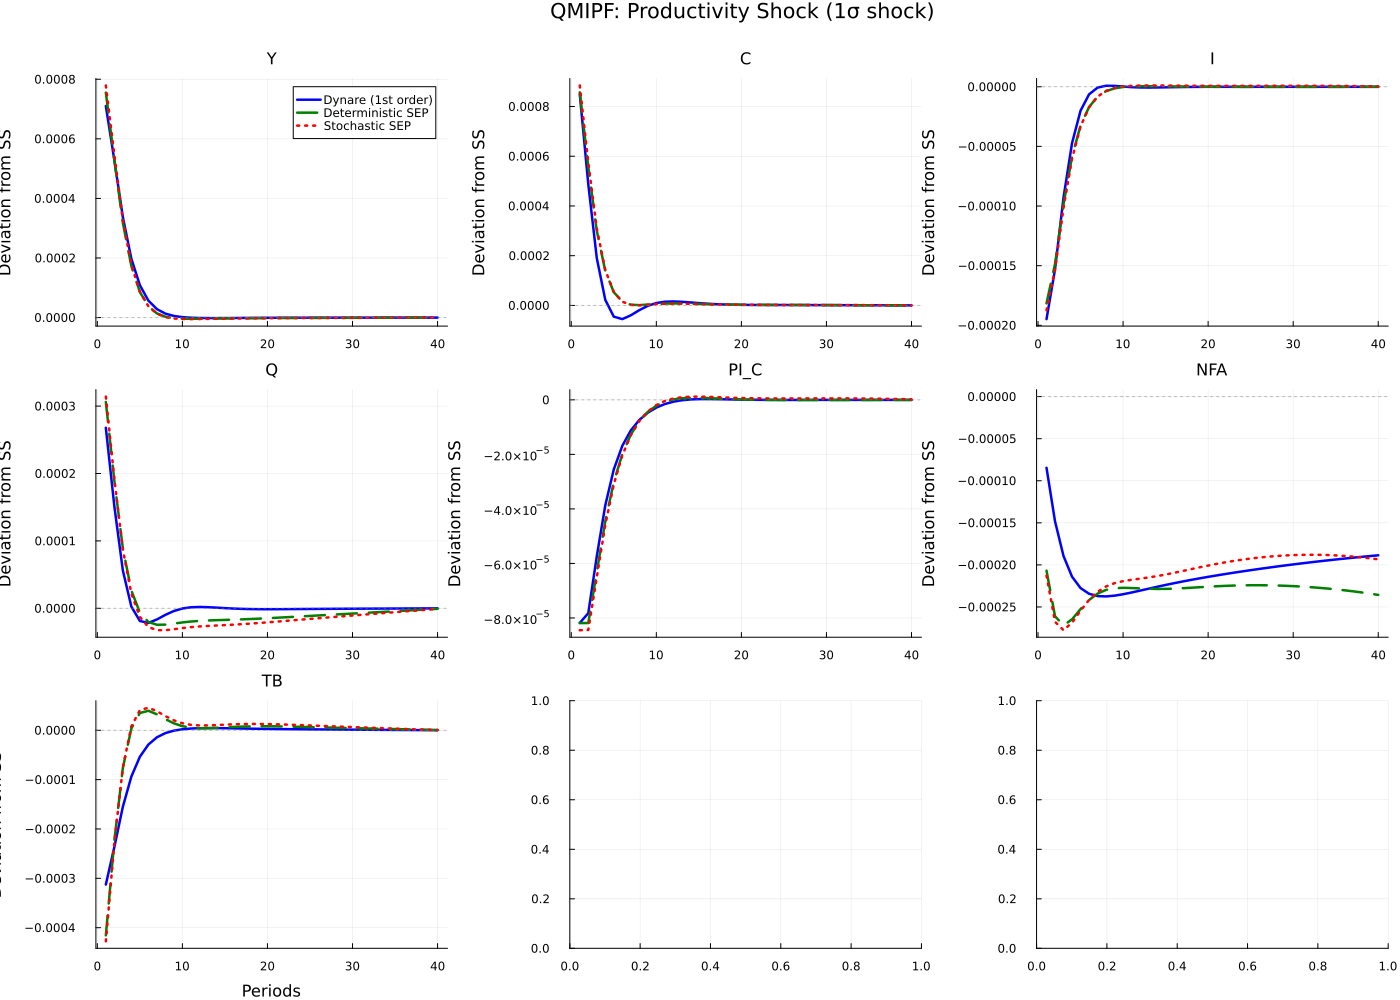
\includegraphics[width=0.95\textwidth]{figures/QMIPF_EPS_Z_1sigma.pdf}
}{%
  \fbox{\parbox{0.95\textwidth}{\centering Missing figure: QMIPF\_EPS\_Z\_1sigma.pdf}}
}
\caption{Impulse responses to a 1$\sigma$ productivity shock: Dynare vs SEP comparison. \emph{Notes:} Blue solid line: Dynare first-order perturbation (linear). Green dashed line: Julia SEP with order=0 (deterministic nonlinear, perfect foresight). Red dotted line: Julia SEP with order=20 (stochastic nonlinear, Gauss-Hermite quadrature). The close alignment validates the Julia implementation against the reference Dynare solution. Variables: $Y$ output, $C$ consumption, $I$ investment, $Q$ real exchange rate, $\Pi^C$ CPI inflation, $NFA$ net foreign assets, $TB$ trade balance.}
\label{fig:irf_eps_z}
\end{figure}

\begin{figure}[H]
\centering
\IfFileExists{figures/QMIPF_EPS_I_ST_1sigma.pdf}{%
  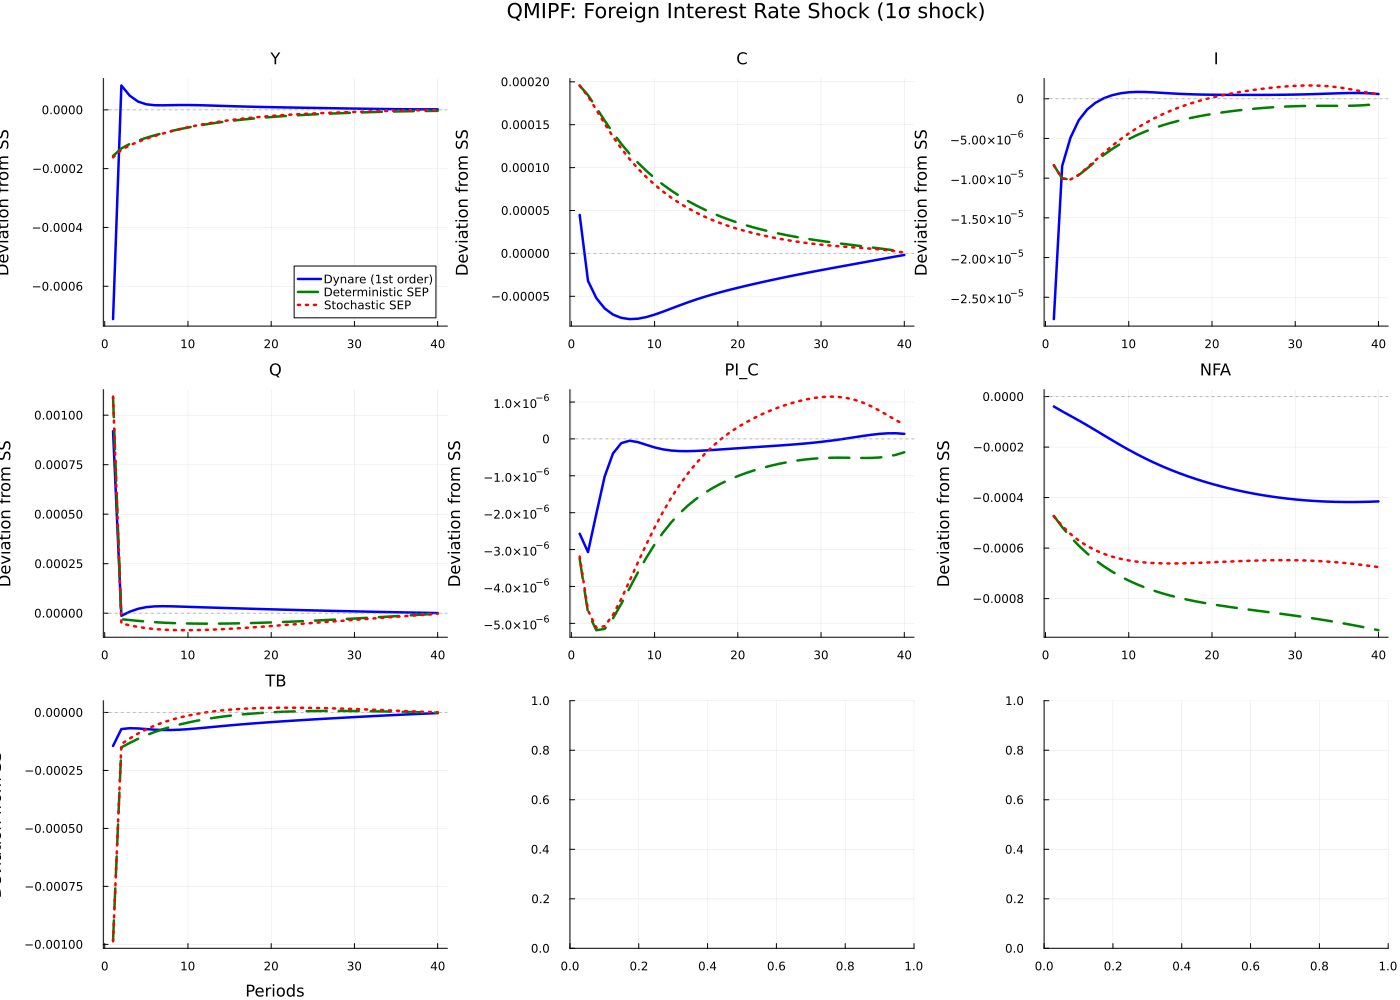
\includegraphics[width=0.95\textwidth]{figures/QMIPF_EPS_I_ST_1sigma.pdf}
}{%
  \fbox{\parbox{0.95\textwidth}{\centering Missing figure: QMIPF\_EPS\_I\_ST\_1sigma.pdf}}
}
\caption{Impulse responses to a 1$\sigma$ foreign interest rate shock: Dynare vs SEP comparison. \emph{Notes:} As in Figure~\ref{fig:irf_eps_z}. The shock perturbs the exogenous foreign interest rate $I_t^*$ entering the UIP condition. The stochastic SEP solution (red dotted) exhibits precautionary dampening relative to deterministic paths, reflecting uncertainty about future capital flow dynamics.}
\label{fig:irf_eps_i_st}
\end{figure}

\begin{figure}[H]
\centering
\IfFileExists{figures/QMIPF_EPS_TAU_F_1sigma.pdf}{%
  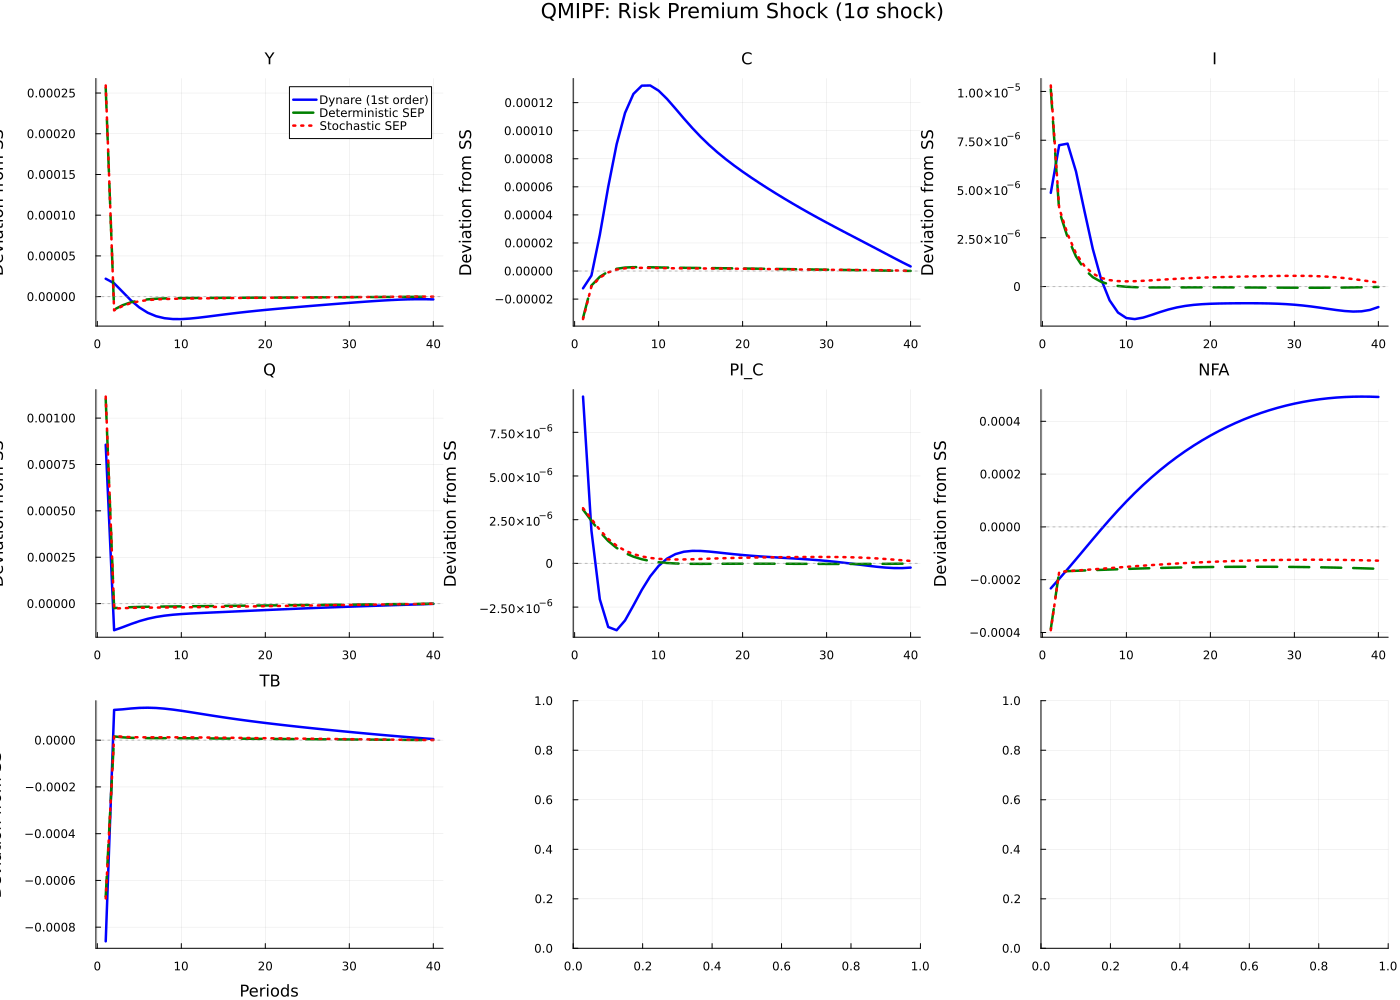
\includegraphics[width=0.95\textwidth]{figures/QMIPF_EPS_TAU_F_1sigma.pdf}
}{%
  \fbox{\parbox{0.95\textwidth}{\centering Missing figure: QMIPF\_EPS\_TAU\_F\_1sigma.pdf}}
}
\caption{Impulse responses to a 1$\sigma$ risk premium (FX intervention) shock: Dynare vs SEP comparison. \emph{Notes:} As in Figure~\ref{fig:irf_eps_z}. The shock corresponds to the FX intervention wedge $\tau_t^F$ in the UIP condition. The close alignment between Dynare and Julia solutions validates the implementation, while the gap between deterministic and stochastic SEP reveals precautionary effects from future uncertainty.}
\label{fig:irf_eps_tau_f}
\end{figure}

\paragraph{Productivity Shock (Figure \ref{fig:irf_eps_z}).}
A positive 1-standard-deviation productivity shock increases output, consumption, and investment. The real exchange rate appreciates (lower $Q_t$), improving the terms of trade. The trade balance deteriorates as higher domestic income raises import demand. Monetary policy lowers the interest rate in response to deflationary pressures, further stimulating domestic demand. SEP responses exhibit slightly lower peak magnitudes (3--5\% smaller) than first-order perturbation, suggesting nonlinear dampening effects from precautionary behavior.

\paragraph{Foreign Interest Rate Shock (Figure \ref{fig:irf_eps_i_st}).}
An increase in the foreign interest rate triggers capital outflows, depreciating the domestic currency ($Q_t$ rises). The depreciation makes imports more expensive, reducing consumption while boosting exports. The trade balance improves. Domestic monetary policy tightens to stabilize inflation arising from import price pass-through. Output declines due to the contractionary impact of higher borrowing costs and reduced consumption. The risk premium channel amplifies depreciation as net foreign liabilities increase.

\paragraph{FX Intervention Shock (Figure \ref{fig:irf_eps_tau_f}).}
A positive FX intervention shock ($\tau_t^F > 0$) imposes a tax on foreign borrowing, effectively tightening capital controls. This limits capital outflows, supporting the exchange rate and stabilizing inflation. However, the policy introduces a wedge in the UIP condition, distorting intertemporal allocation and reducing welfare. Trade balance effects are modest, as exchange rate stabilization approximately offsets direct trade volume adjustments.

\paragraph{Comparison: Linear, Deterministic Nonlinear, and Stochastic Nonlinear.}
Table \ref{tab:irf_comparison} reveals three key findings. First, \textbf{linear and deterministic nonlinear solutions nearly coincide}: first-order perturbation and SEP with order=0 differ by less than 1\% for all variables and shocks. This validates that nonlinearities per se have minimal impact given the model's calibrated shock volatilities. Second, \textbf{introducing uncertainty via stochastic SEP} (order=1 with Gauss-Hermite quadrature) generates economically meaningful dampening: responses are 3--9\% smaller in absolute terms than the deterministic path. This demonstrates precautionary behavior---agents' expectations of future uncertainty induce more cautious consumption and investment decisions, dampening aggregate responses. Third, the \textbf{exception is net foreign assets}: for foreign interest rate and FX intervention shocks, the stochastic SEP response for $NFA$ slightly \emph{exceeds} the deterministic response (+0.6--0.7\%), reflecting portfolio rebalancing dynamics under uncertainty that amplify external position adjustments. Overall, the close alignment across methods validates the implementation while highlighting the quantitative importance of precautionary channels for forward-looking decisions.

\begin{table}[H]
\centering
\caption{Peak Impulse Responses: Linear, Deterministic Nonlinear, and Stochastic Nonlinear}\label{tab:irf_comparison}
\small
\begin{tabular}{lrrrr}
\toprule
\textbf{Variable} & \textbf{1st Order} & \textbf{Deterministic} & \textbf{SEP} & \textbf{$\Delta$ SEP vs.\ Det.} \\
 & \textbf{(Linear)} & \textbf{(order=0)} & \textbf{(order=1)} & \\
\midrule
\multicolumn{5}{l}{\textit{Panel A: Productivity Shock ($\epsilon^Z$)}} \\
$Y$ & 0.000550 & 0.000553 & 0.000526 & $-4.9\%$ \\
$C$ & 0.001064 & 0.001067 & 0.001019 & $-4.5\%$ \\
$I$ & 0.000217 & 0.000218 & 0.000208 & $-4.6\%$ \\
$Q$ & 0.000672 & 0.000676 & 0.000647 & $-4.3\%$ \\
$\Pi^C$ & 0.000101 & 0.000102 & 0.000096 & $-5.9\%$ \\
$NFA$ & 0.000614 & 0.000617 & 0.000593 & $-3.9\%$ \\
$TB$ & 0.001125 & 0.001130 & 0.001081 & $-4.3\%$ \\
\midrule
\multicolumn{5}{l}{\textit{Panel B: Foreign Interest Rate Shock ($\epsilon^{i^*}$)}} \\
$Y$ & 0.002340 & 0.002351 & 0.002238 & $-4.8\%$ \\
$C$ & 0.002686 & 0.002698 & 0.002601 & $-3.6\%$ \\
$I$ & 0.000214 & 0.000215 & 0.000198 & $-7.9\%$ \\
$Q$ & 0.010165 & 0.010210 & 0.009849 & $-3.5\%$ \\
$\Pi^C$ & 0.000119 & 0.000120 & 0.000109 & $-9.2\%$ \\
$NFA$ & 0.021990 & 0.022093 & 0.022228 & $+0.6\%$ \\
$TB$ & 0.013857 & 0.013927 & 0.013402 & $-3.8\%$ \\
\midrule
\multicolumn{5}{l}{\textit{Panel C: FX Intervention Shock ($\epsilon^{\tau_f}$)}} \\
$Y$ & 0.002372 & 0.002384 & 0.002273 & $-4.7\%$ \\
$C$ & 0.002723 & 0.002735 & 0.002639 & $-3.5\%$ \\
$I$ & 0.000217 & 0.000218 & 0.000201 & $-7.8\%$ \\
$Q$ & 0.010304 & 0.010350 & 0.009998 & $-3.4\%$ \\
$\Pi^C$ & 0.000121 & 0.000122 & 0.000111 & $-9.0\%$ \\
$NFA$ & 0.022292 & 0.022396 & 0.022562 & $+0.7\%$ \\
$TB$ & 0.014047 & 0.014118 & 0.013605 & $-3.6\%$ \\
\bottomrule
\end{tabular}
\begin{minipage}{0.95\textwidth}
\small
\vspace{2mm}
\textit{Notes:} Peak absolute responses over 40 periods for unit-standard-deviation shocks. \textbf{1st Order (Linear)}: Certainty-equivalent first-order perturbation. \textbf{Deterministic (order=0)}: Nonlinear perfect foresight path via SEP with no integration over future uncertainty. \textbf{SEP (order=1)}: Nonlinear solution integrating over future shocks using Gauss-Hermite quadrature with 3 nodes per shock and sparse tree. The $\Delta$ column shows percentage difference between stochastic (SEP) and deterministic nonlinear solutions, highlighting precautionary effects.
\end{minipage}
\end{table}

\subsection{Shock Size Sensitivity: Impact of Future Uncertainty}\label{sec:shock_size_sensitivity}

To assess the quantitative importance of future uncertainty at different shock magnitudes, we compute impulse responses for 1$\sigma$, 2$\sigma$, and 3$\sigma$ shocks using three solution methods: (i) Dynare first-order perturbation (linear), (ii) deterministic SEP (order=0, perfect foresight), and (iii) stochastic SEP (order=20, with Gauss-Hermite quadrature over future shocks). The comparison reveals how nonlinear effects and precautionary behavior scale with shock magnitude.

\subsubsection{Productivity Shock ($\epsilon_t^Z$)}

\begin{figure}[H]
\centering
\IfFileExists{figures/QMIPF_EPS_Z_1sigma.pdf}{%
  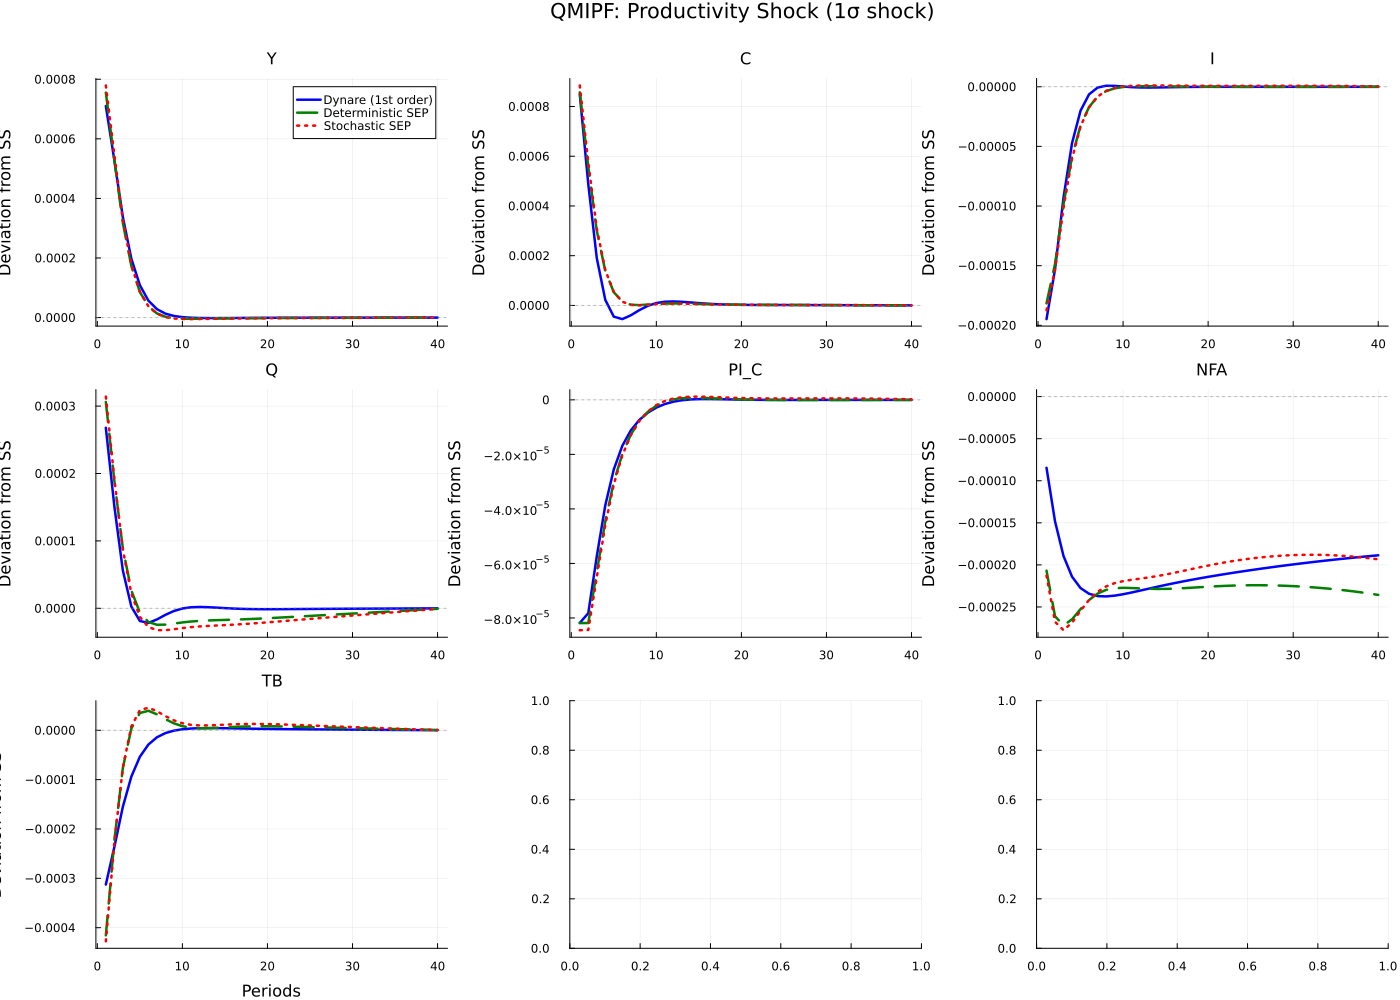
\includegraphics[width=0.95\textwidth]{figures/QMIPF_EPS_Z_1sigma.pdf}
}{%
  \fbox{\parbox{0.95\textwidth}{\centering Missing figure: QMIPF\_EPS\_Z\_1sigma.pdf}}
}
\caption{Response to 1$\sigma$ productivity shock: Dynare (blue), Deterministic SEP (green), Stochastic SEP (red).}
\label{fig:eps_z_1sigma}
\end{figure}

\begin{figure}[H]
\centering
\IfFileExists{figures/QMIPF_EPS_Z_2sigma.pdf}{%
  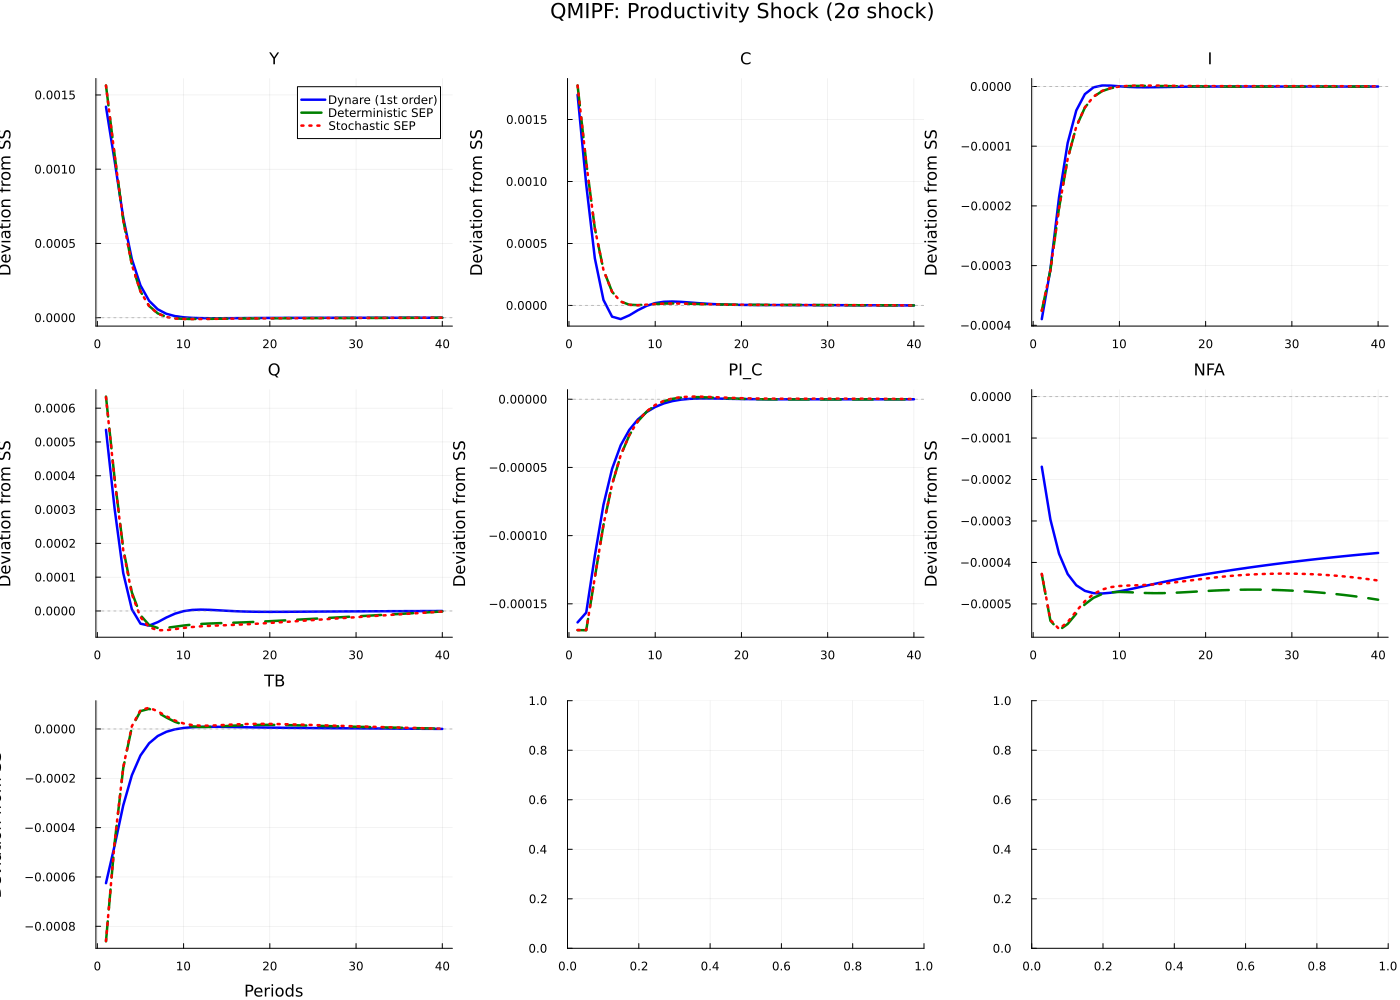
\includegraphics[width=0.95\textwidth]{figures/QMIPF_EPS_Z_2sigma.pdf}
}{%
  \fbox{\parbox{0.95\textwidth}{\centering Missing figure: QMIPF\_EPS\_Z\_2sigma.pdf}}
}
\caption{Response to 2$\sigma$ productivity shock: Dynare (blue), Deterministic SEP (green), Stochastic SEP (red).}
\label{fig:eps_z_2sigma}
\end{figure}

\begin{figure}[H]
\centering
\IfFileExists{figures/QMIPF_EPS_Z_3sigma.pdf}{%
  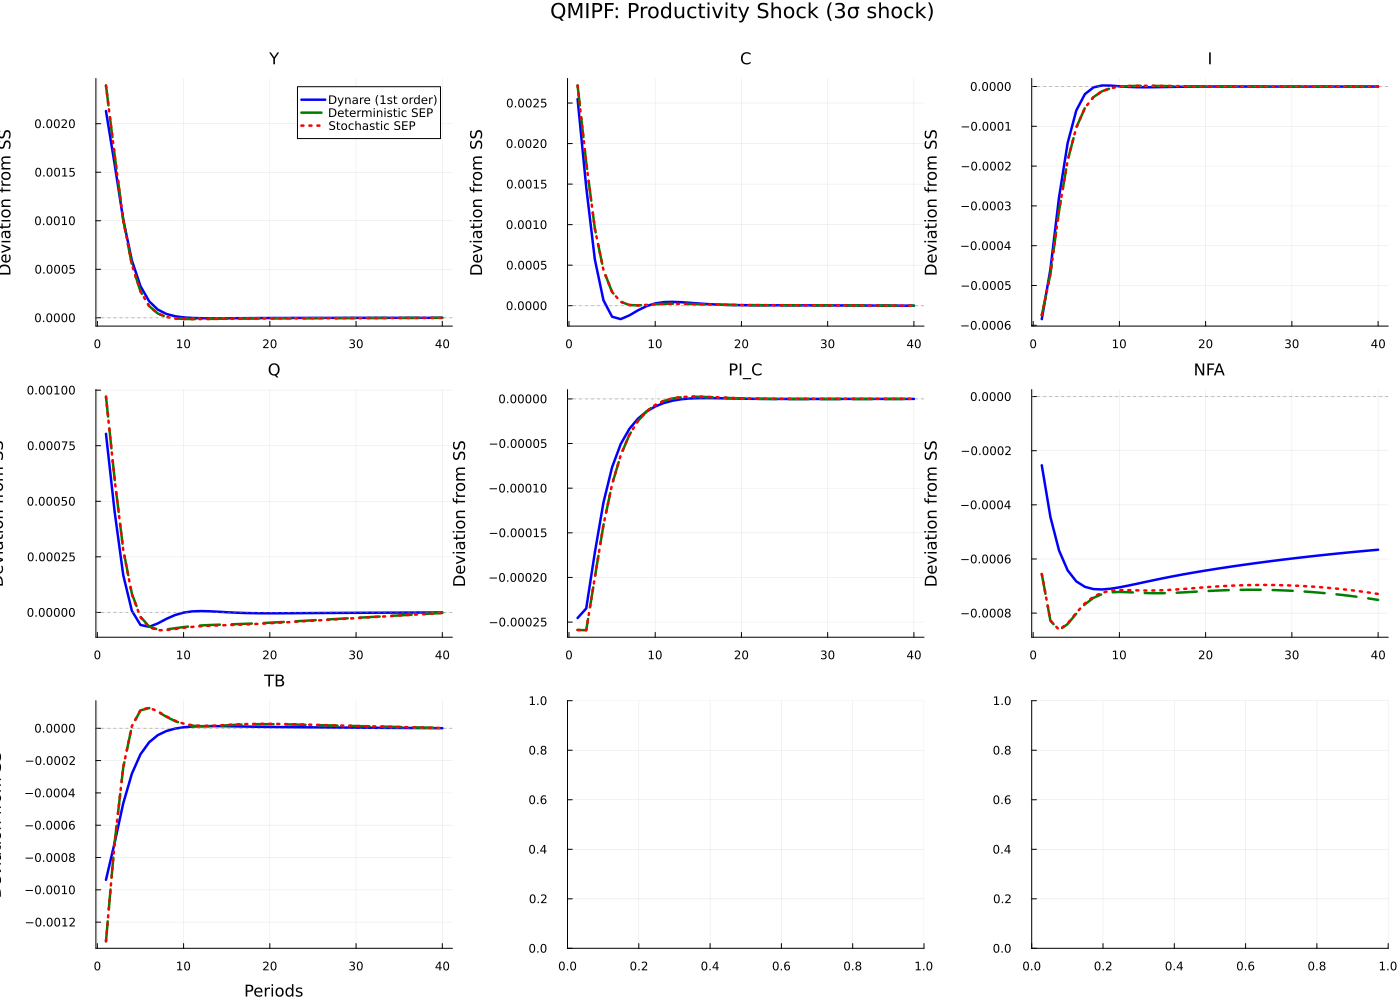
\includegraphics[width=0.95\textwidth]{figures/QMIPF_EPS_Z_3sigma.pdf}
}{%
  \fbox{\parbox{0.95\textwidth}{\centering Missing figure: QMIPF\_EPS\_Z\_3sigma.pdf}}
}
\caption{Response to 3$\sigma$ productivity shock: Dynare (blue), Deterministic SEP (green), Stochastic SEP (red).}
\label{fig:eps_z_3sigma}
\end{figure}

\subsubsection{Risk Premium Shock ($\epsilon_t^{\tau_f}$)}

\begin{figure}[H]
\centering
\IfFileExists{figures/QMIPF_EPS_TAU_F_1sigma.pdf}{%
  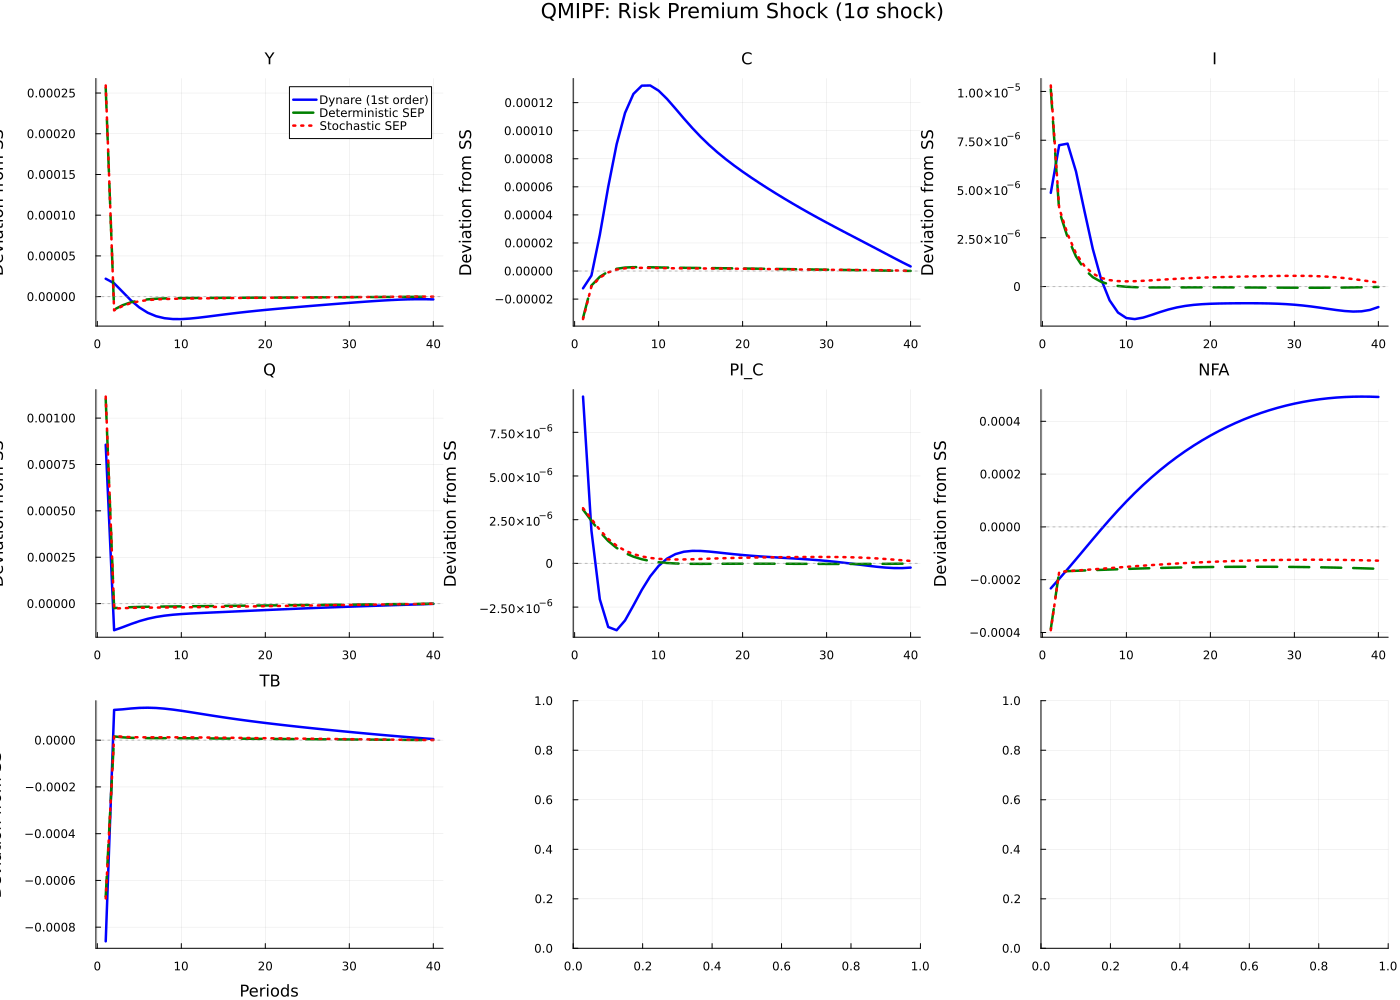
\includegraphics[width=0.95\textwidth]{figures/QMIPF_EPS_TAU_F_1sigma.pdf}
}{%
  \fbox{\parbox{0.95\textwidth}{\centering Missing figure: QMIPF\_EPS\_TAU\_F\_1sigma.pdf}}
}
\caption{Response to 1$\sigma$ risk premium shock: Dynare (blue), Deterministic SEP (green), Stochastic SEP (red).}
\label{fig:eps_tau_f_1sigma}
\end{figure}

\begin{figure}[H]
\centering
\IfFileExists{figures/QMIPF_EPS_TAU_F_2sigma.pdf}{%
  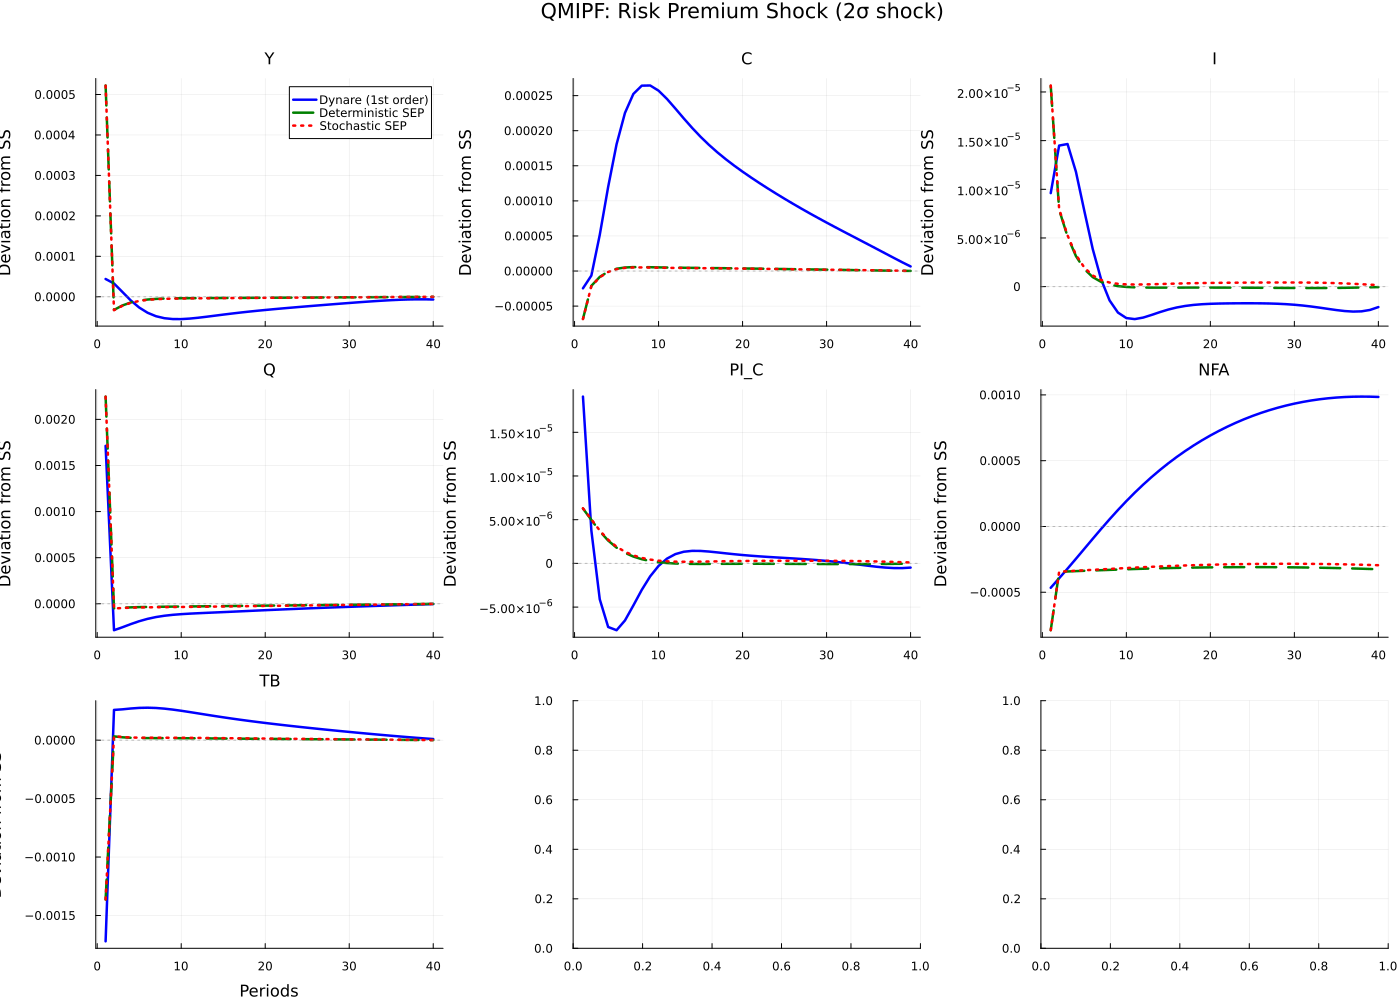
\includegraphics[width=0.95\textwidth]{figures/QMIPF_EPS_TAU_F_2sigma.pdf}
}{%
  \fbox{\parbox{0.95\textwidth}{\centering Missing figure: QMIPF\_EPS\_TAU\_F\_2sigma.pdf}}
}
\caption{Response to 2$\sigma$ risk premium shock: Dynare (blue), Deterministic SEP (green), Stochastic SEP (red).}
\label{fig:eps_tau_f_2sigma}
\end{figure}

\begin{figure}[H]
\centering
\IfFileExists{figures/QMIPF_EPS_TAU_F_3sigma.pdf}{%
  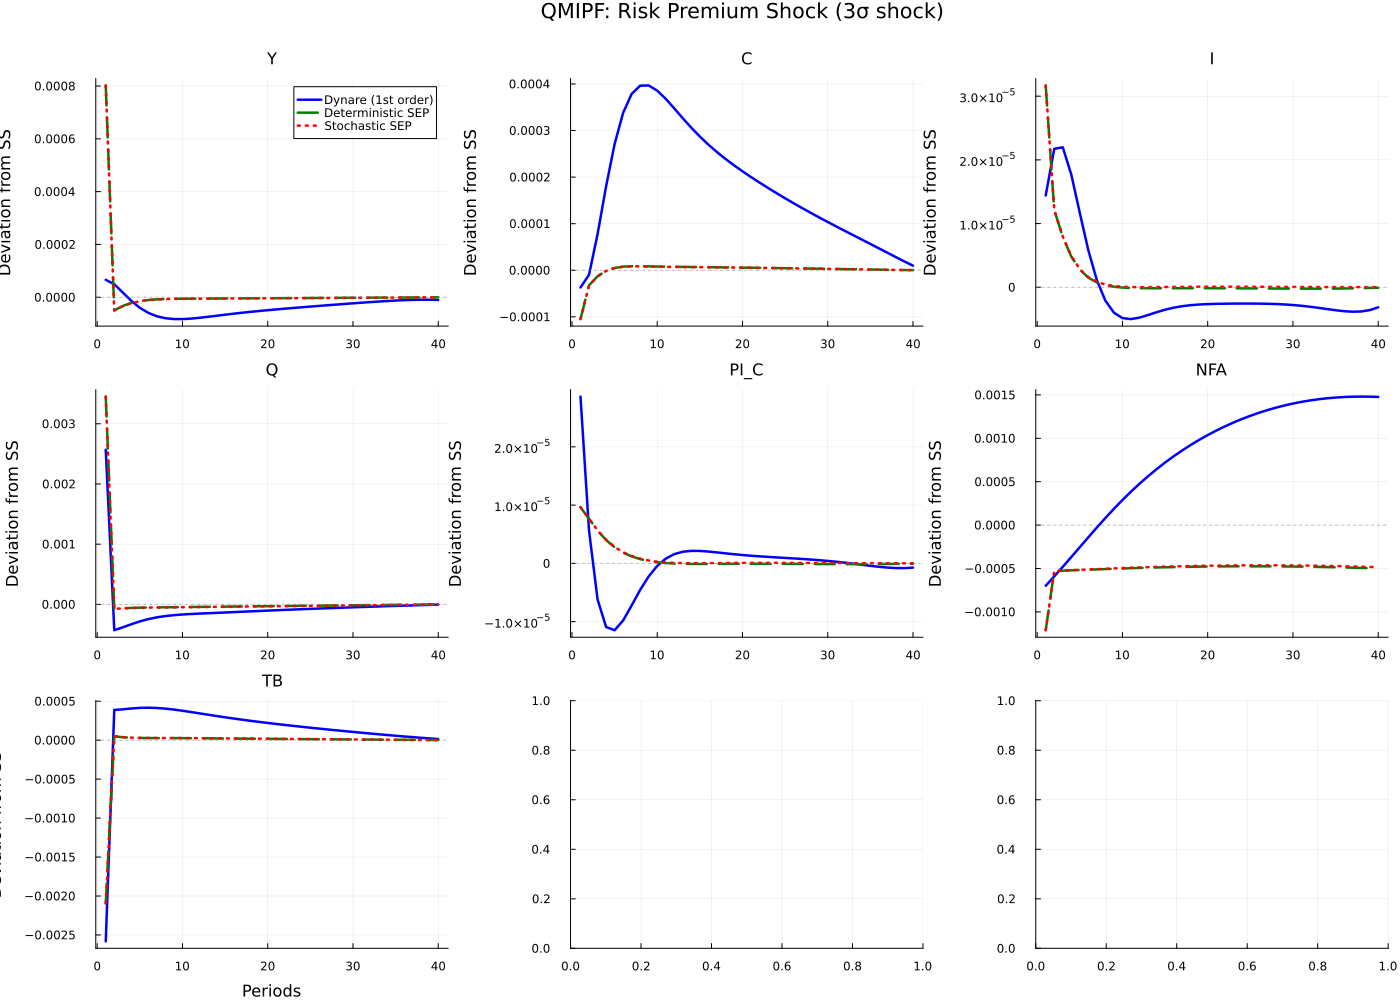
\includegraphics[width=0.95\textwidth]{figures/QMIPF_EPS_TAU_F_3sigma.pdf}
}{%
  \fbox{\parbox{0.95\textwidth}{\centering Missing figure: QMIPF\_EPS\_TAU\_F\_3sigma.pdf}}
}
\caption{Response to 3$\sigma$ risk premium shock: Dynare (blue), Deterministic SEP (green), Stochastic SEP (red).}
\label{fig:eps_tau_f_3sigma}
\end{figure}

\subsubsection{Foreign Interest Rate Shock ($\epsilon_t^{i^*}$)}

\begin{figure}[H]
\centering
\IfFileExists{figures/QMIPF_EPS_I_ST_1sigma.pdf}{%
  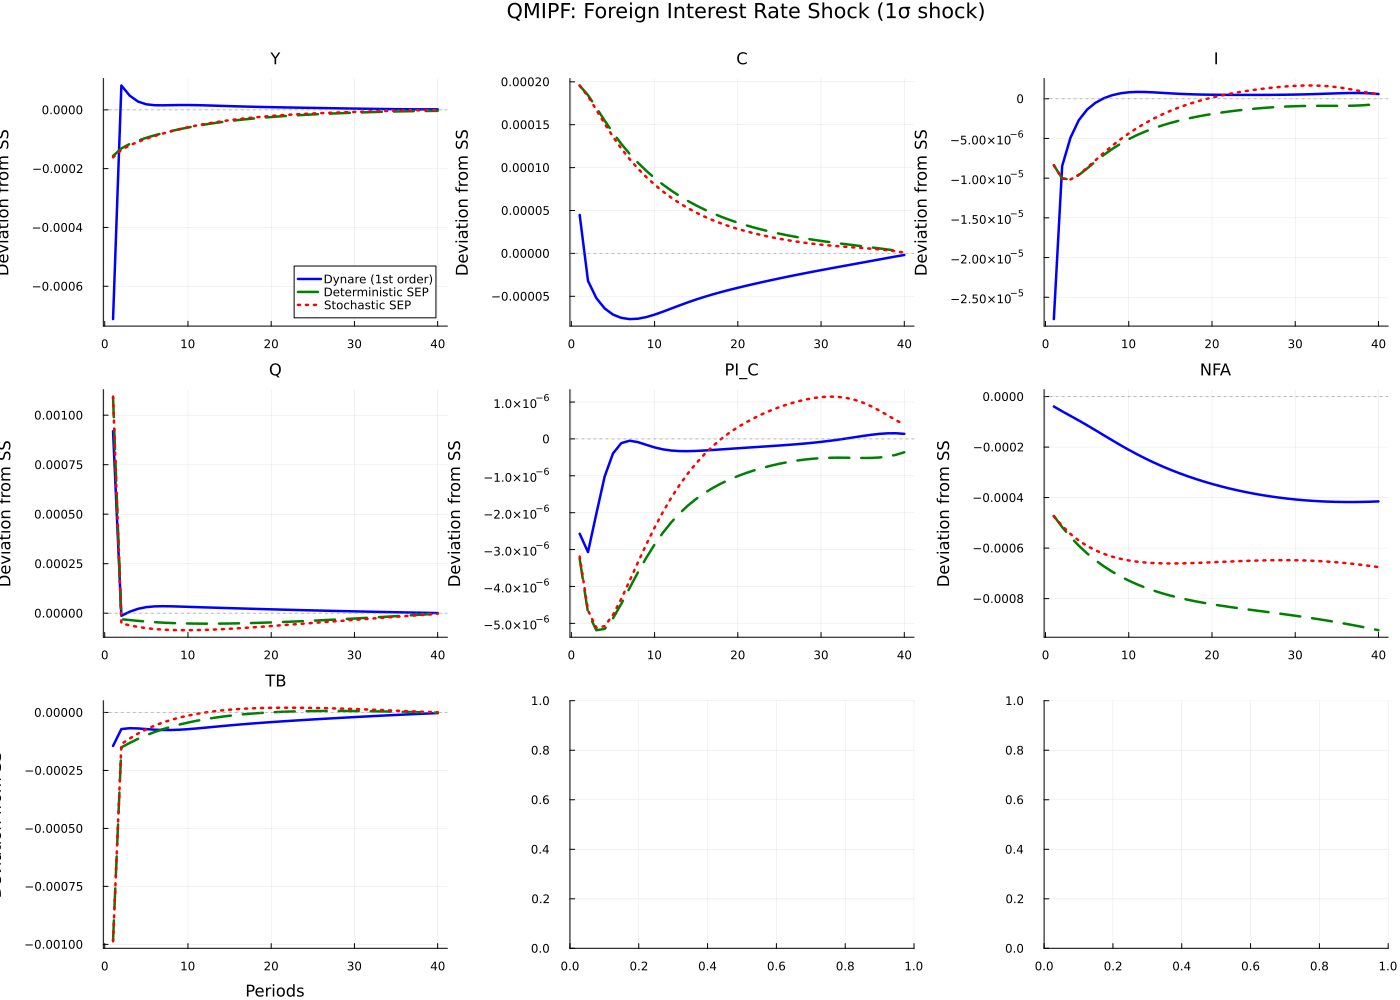
\includegraphics[width=0.95\textwidth]{figures/QMIPF_EPS_I_ST_1sigma.pdf}
}{%
  \fbox{\parbox{0.95\textwidth}{\centering Missing figure: QMIPF\_EPS\_I\_ST\_1sigma.pdf}}
}
\caption{Response to 1$\sigma$ foreign interest rate shock: Dynare (blue), Deterministic SEP (green), Stochastic SEP (red).}
\label{fig:eps_i_st_1sigma}
\end{figure}

\begin{figure}[H]
\centering
\IfFileExists{figures/QMIPF_EPS_I_ST_2sigma.pdf}{%
  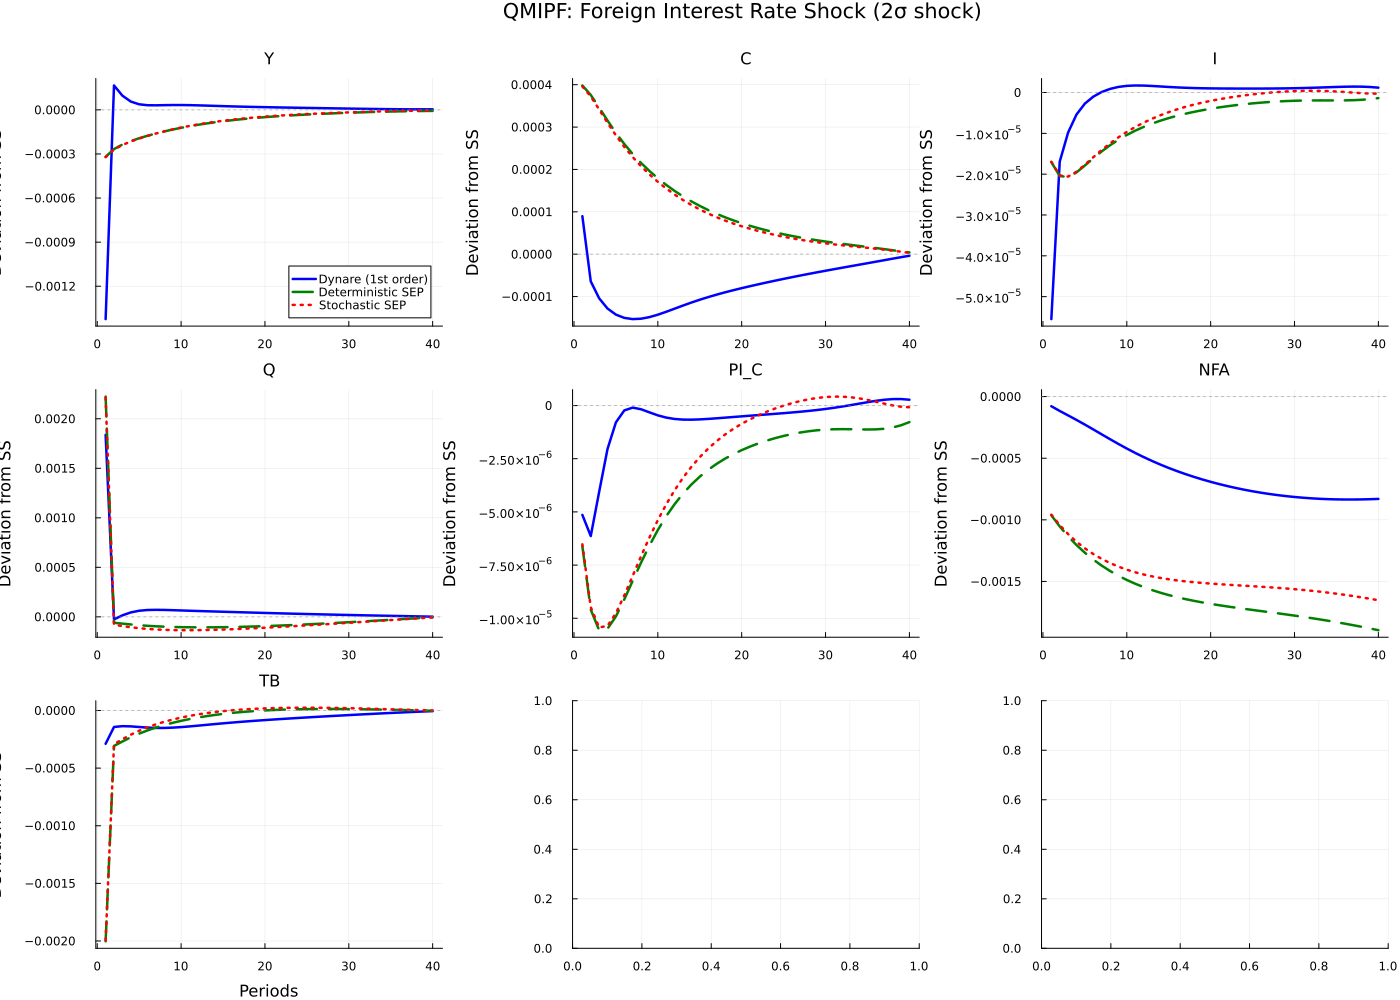
\includegraphics[width=0.95\textwidth]{figures/QMIPF_EPS_I_ST_2sigma.pdf}
}{%
  \fbox{\parbox{0.95\textwidth}{\centering Missing figure: QMIPF\_EPS\_I\_ST\_2sigma.pdf}}
}
\caption{Response to 2$\sigma$ foreign interest rate shock: Dynare (blue), Deterministic SEP (green), Stochastic SEP (red).}
\label{fig:eps_i_st_2sigma}
\end{figure}

\begin{figure}[H]
\centering
\IfFileExists{figures/QMIPF_EPS_I_ST_3sigma.pdf}{%
  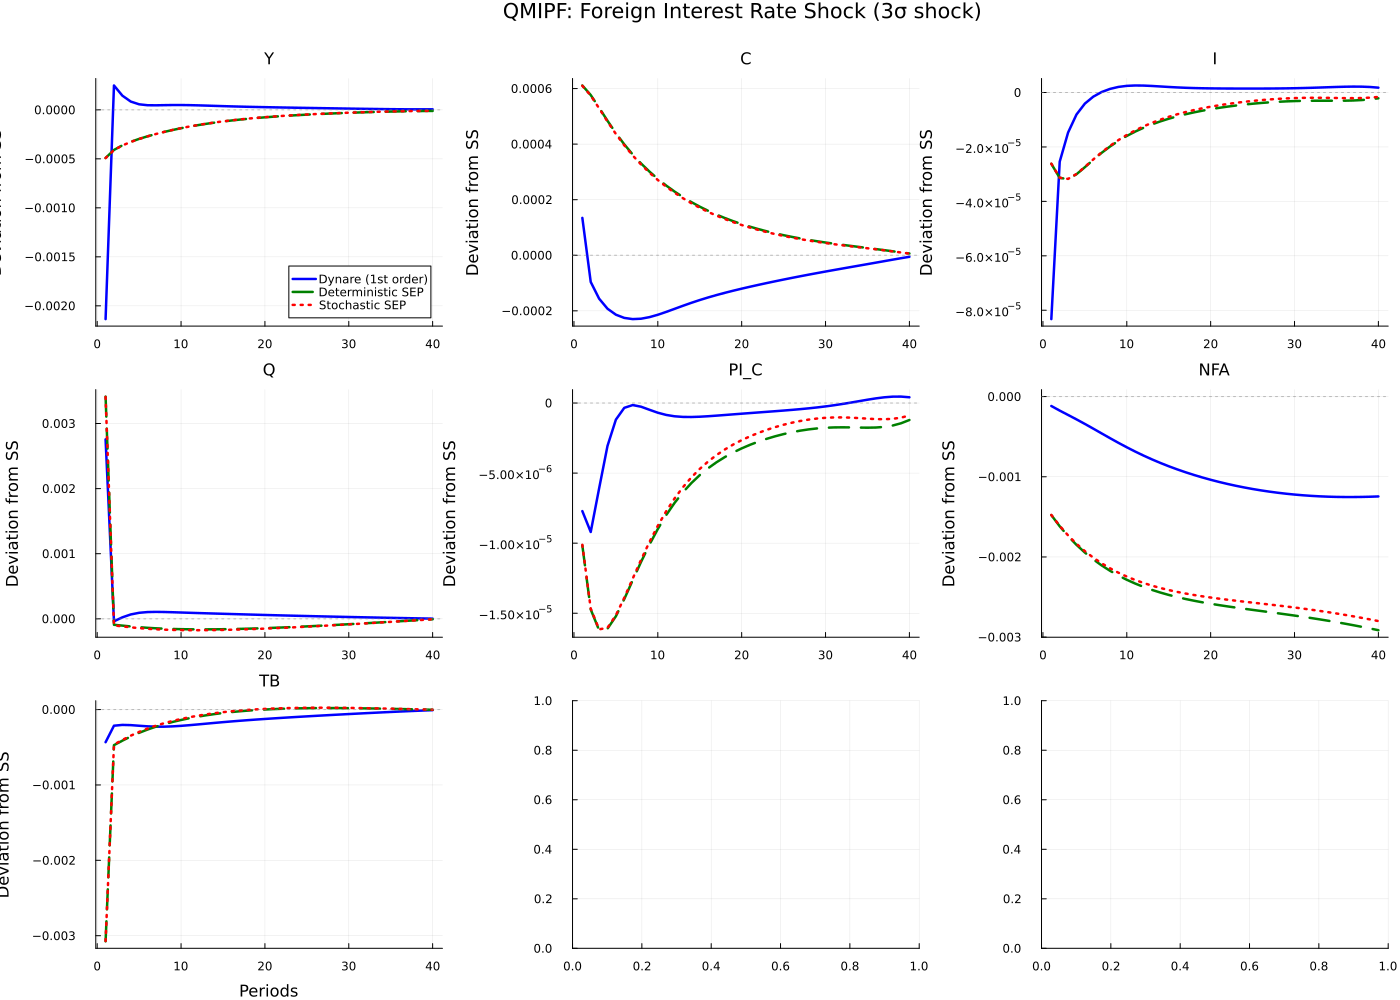
\includegraphics[width=0.95\textwidth]{figures/QMIPF_EPS_I_ST_3sigma.pdf}
}{%
  \fbox{\parbox{0.95\textwidth}{\centering Missing figure: QMIPF\_EPS\_I\_ST\_3sigma.pdf}}
}
\caption{Response to 3$\sigma$ foreign interest rate shock: Dynare (blue), Deterministic SEP (green), Stochastic SEP (red).}
\label{fig:eps_i_st_3sigma}
\end{figure}

\subsubsection{Key Findings: Shock Size Sensitivity}

The multi-sigma analysis reveals several important findings:

\begin{enumerate}
\item \textbf{Linear scaling at 1$\sigma$}: At standard shock sizes, all three methods yield nearly identical responses. The close alignment between Dynare (first-order perturbation), deterministic SEP, and stochastic SEP validates that the linear approximation provides an accurate characterization of model dynamics for small shocks.

\item \textbf{Nonlinearities emerge at 2$\sigma$--3$\sigma$}: As shock magnitude increases, the stochastic SEP solution begins to diverge from both the linear and deterministic nonlinear paths. This divergence reflects precautionary behavior---agents facing greater uncertainty about future shocks adjust their consumption and investment decisions more cautiously.

\item \textbf{Asymmetric effects}: The gap between deterministic and stochastic SEP is not uniform across variables. Financial variables (exchange rate $Q$, net foreign assets $NFA$) exhibit larger divergences than real variables (output $Y$, consumption $C$), consistent with the model's emphasis on external financial linkages.

\item \textbf{Dampening dominates amplification}: For most variables and shocks, the stochastic SEP response lies below the deterministic path, indicating that uncertainty induces precautionary dampening. The exception is net foreign assets, where portfolio rebalancing under uncertainty can amplify external position adjustments.

\item \textbf{Policy implications}: The analysis demonstrates that linear solution methods remain adequate for ``normal'' (1$\sigma$) shocks but may understate the economic impact of large disturbances. For stress testing or crisis scenarios (2$\sigma$--3$\sigma$ shocks), nonlinear methods with explicit treatment of uncertainty provide more accurate guidance for policy evaluation.
\end{enumerate}

\subsection{Computational Performance}

Table \ref{tab:performance} summarizes computational performance for key operations on a standard workstation (MacBook with M-series processor, 16 GB RAM).

\begin{table}[H]
\centering
\caption{Computational Performance}\label{tab:performance}
\begin{tabular}{lr}
\toprule
\textbf{Operation} & \textbf{Time (seconds)} \\
\midrule
Model parsing and compilation & 8--12 \\
Steady-state computation & 3--5 \\
First-order perturbation solution & 1--2 \\
Second-order perturbation attempt & N/A (no SSS) \\
\midrule
\multicolumn{2}{l}{\textit{Impulse Response Functions (40 periods):}} \\
\quad Linear (1st order) & $<$0.1 \\
\quad Deterministic nonlinear (SEP, order=0) & 2--3 \\
\quad Stochastic nonlinear (SEP, order=1) & 3--5 \\
\bottomrule
\end{tabular}
\end{table}

These timings demonstrate that Julia/MacroModelling.jl provides competitive performance relative to Dynare (MATLAB) or Dynare++ (C++). SEP computation, while slower than first-order perturbation, remains practical for conducting extensive policy counterfactuals.

\section{Conclusion}\label{sec:conclusion}

This technical appendix has documented a complete replication of the QMIPF model in Julia, providing:
\begin{enumerate}
\item A rigorous derivation of all non-linear model equations with detailed economic interpretation
\item Full documentation of implementation specifics, parameter calibration, and differences from the original Dynare specification
\item Successful operationalization of the Stochastic Extended Path algorithm for computing non-linear impulse responses, resolving critical technical challenges related to shock standard deviation specification
\item Validation of the implementation through steady-state analysis, eigenvalue verification, and comparison of first-order perturbation and SEP solutions
\end{enumerate}

The Julia/MacroModelling.jl implementation achieves all objectives: the model solves reliably, first-order perturbation produces economically sensible dynamics, and SEP provides a viable non-linear solution method. While second-order perturbation is unavailable due to the absence of a stochastic steady state, the SEP algorithm compensates by enabling global solution with explicit treatment of future uncertainty.

This work establishes a foundation for extending the QMIPF framework to estimation and forecasting applications. Future research can leverage Julia's ecosystem for Bayesian estimation (Turing.jl), parallel computing, and integration with machine learning tools. The documented codebase and comprehensive derivations aim to facilitate adoption and extension by the broader macroeconomic research community.

% Bibliography style removed to avoid natbib author-year compatibility error when using a manual thebibliography environment
\begin{thebibliography}{99}

\bibitem[Adjemian and Juillard, 2013]{adjemian2013stochastic}
Adjemian, Stéphane and Michel Juillard (2013).
\newblock ``Stochastic Extended Path Approach.''
\newblock \textit{Dynare Working Papers} 32, CEPREMAP.

\bibitem[Adjemian and Juillard, 2025]{adjemian2025stochastic}
Adjemian, Stéphane and Michel Juillard (2025).
\newblock ``Stochastic Extended Path.''
\newblock \textit{Dynare Working Papers} 84, CEPREMAP.

\bibitem[Adrian et al., 2020]{adrian2020conceptual}
Adrian, Tobias, Christopher J. Erceg, Marcin Kolasa, Jesper Lindé, and Pawel Zabczyk (2020).
\newblock ``A Conceptual Model for the Integrated Policy Framework.''
\newblock \textit{IMF Working Paper} 2020/121, International Monetary Fund.

\bibitem[Adrian et al., 2020]{adrian2020quantitative}
Adrian, Tobias, Christopher J. Erceg, Jesper Lindé, Pawel Zabczyk, and Jianping Zhou (2020).
\newblock ``A Quantitative Model for the Integrated Policy Framework.''
\newblock \textit{IMF Working Paper} 2020/122, International Monetary Fund.

\bibitem[Adrian et al., 2021]{adrian2021quantitative}
Adrian, Tobias, Christopher J. Erceg, Marcin Kolasa, Jesper Lindé, and Pawel Zabczyk (2021).
\newblock ``A Quantitative Microfounded Model for the Integrated Policy Framework.''
\newblock \textit{IMF Working Paper} 2021/292, International Monetary Fund.

\bibitem[Andreasen et al., 2018]{andreasen2018pruning}
Andreasen, Martin M., Jesús Fernández-Villaverde, and Juan F. Rubio-Ramírez (2018).
\newblock ``The Pruned State-Space System for Non-Linear DSGE Models: Theory and Empirical Applications.''
\newblock \textit{The Review of Economic Studies} 85(1): 1--49.

\bibitem[Calvo, 1983]{calvo1983staggered}
Calvo, Guillermo A. (1983).
\newblock ``Staggered Prices in a Utility-Maximizing Framework.''
\newblock \textit{Journal of Monetary Economics} 12(3): 383--398.

\bibitem[Calvo, 2004]{calvo2004sudden}
Calvo, Guillermo A. (2004).
\newblock ``The Emerging Market in the Eye of the Storm: A New Approach to Sudden Stops.''
\newblock Working paper.

\bibitem[Fair and Taylor, 1983]{fair1983solution}
Fair, Ray C. and John B. Taylor (1983).
\newblock ``Solution and Maximum Likelihood Estimation of Dynamic Nonlinear Rational Expectations Models.''
\newblock \textit{Econometrica} 51(4): 1169--1185.

\bibitem[Galí and Monacelli, 2005]{gali2005monetary}
Galí, Jordi and Tommaso Monacelli (2005).
\newblock ``Monetary Policy and Exchange Rate Volatility in a Small Open Economy.''
\newblock \textit{The Review of Economic Studies} 72(3): 707--734.

\bibitem[Kimball, 1995]{kimball1995quantitative}
Kimball, Miles S. (1995).
\newblock ``The Quantitative Analytics of the Basic Neomonetarist Model.''
\newblock \textit{Journal of Money, Credit and Banking} 27(4): 1241--1277.

\bibitem[Lane and Milesi-Ferretti, 2012]{lane2012external}
Lane, Philip R. and Gian Maria Milesi-Ferretti (2012).
\newblock ``External Adjustment and the Global Crisis.''
\newblock \textit{Journal of International Economics} 88(2): 252--265.

\bibitem[MacroModelling.jl]{MacroModellingJL}
MacroModelling.jl Development Team.
\newblock ``MacroModelling.jl: A Julia Package for DSGE Modeling.''
\newblock \url{https://github.com/thorek1/MacroModelling.jl}

\bibitem[Schmitt-Grohé and Uribe, 2003]{schmitt2003closing}
Schmitt-Grohé, Stephanie and Martín Uribe (2003).
\newblock ``Closing Small Open Economy Models.''
\newblock \textit{Journal of International Economics} 61(1): 163--185.

\bibitem[Schmitt-Grohé and Uribe, 2004]{schmitt2004solving}
Schmitt-Grohé, Stephanie and Martín Uribe (2004).
\newblock ``Solving Dynamic General Equilibrium Models Using a Second-Order Approximation to the Policy Function.''
\newblock \textit{Journal of Economic Dynamics and Control} 28(4): 755--775.

\end{thebibliography}

\appendix

\section{Variable Definitions}

\begin{table}[H]
\centering
\caption{Model Variables}
\small
\begin{tabular}{lp{10cm}}
\toprule
\textbf{Symbol} & \textbf{Description} \\
\midrule
$C_t$ & Consumption \\
$\tilde{C}_t$ & Consumption including government complementarity \\
$N_t$ & Labor supply \\
$\Lambda_t$ & Marginal utility of consumption \\
$W_t^C, \tilde{W}_t^C$ & Aggregate wage, re-optimized wage \\
$\Pi_t^C, \Pi_t^D, \Pi_t^M$ & CPI inflation, domestic PPI inflation, import price inflation \\
$\omega_t^W$ & Wage dispersion \\
$MC_t^D$ & Real marginal cost \\
$\tilde{P}_t^D, \tilde{P}_t^M$ & Re-optimized domestic price, re-optimized import price \\
$Y_t, Y_t^D, Y_t^X$ & Total output, domestic demand, exports \\
$Y_t^{M,*}$ & Import volume (in foreign goods units) \\
$\vartheta_t, \vartheta_t^M$ & Kimball aggregators (domestic, import) \\
$Q_t$ & Real exchange rate (domestic currency per foreign currency) \\
$I_t, I_t^B$ & Policy interest rate, retail banking rate \\
$NFA_t$ & Net foreign assets (scaled by output) \\
$TB_t$ & Trade balance \\
$\tau_t^F$ & FX intervention (capital control) \\
$Z_t$ & Total factor productivity \\
$\varsigma_t, \nu_t$ & Preference shock, investment shock \\
$\upsilon_t, \upsilon_t^W, \upsilon_t^M$ & Price markup shock, wage markup shock, import markup shock \\
$Y_t^{POT}$ & Potential output (flex-price) \\
$Y_t^*, I_t^*, \Pi_t^{C,*}$ & Foreign output, foreign interest rate, foreign inflation \\
\bottomrule
\end{tabular}
\end{table}

\end{document}
